\documentclass[11pt,a4paper]{article}

% ---------- Packages ----------
\usepackage[utf8]{inputenc}
\usepackage[T1]{fontenc}
\usepackage[lining]{gelasio}
\usepackage[margin=2.5cm]{geometry}
\usepackage{graphicx}
\usepackage{booktabs}
\usepackage{amsmath}
\usepackage{float}
\usepackage{caption}
\usepackage{hyperref}
\usepackage{amssymb}
\usepackage{pdfpages}
\usepackage{setspace}
\usepackage{xcolor}
\hypersetup{colorlinks=true, linkcolor=blue, citecolor=blue, urlcolor=blue}
\setlength{\parskip}{0.5em}
\setlength{\parindent}{0pt}

\begin{document}

\begin{titlepage}
  \centering
  \vspace*{2cm}
  {\LARGE\bfseries Distributed LLM Inference on the Edge:\\[0.4em]
   Parallelism, Network and Bottlenecks\\[0.4em]
   on a Raspberry Pi Cluster\par}
  \vspace{2cm}
  {\large Project Report\par}
  {\large Supervisors: Yixing Zhang and Romaric Duvignau\par}
  {\large Group: 7\par}
  \vspace{1.5cm}
  {\large Yuzhou Zhang\\ Yunfan Zhang\\ Shuo Zhang\\ Wenqi Zhao\par}
  \vfill
  {\large Chalmers University of Technology\\
   Gothenburg, Sweden\par}
  \vspace{0.5cm}
  {\large \today\par}
\end{titlepage}

% ---------- Abstract ----------
\begin{abstract}
Running large language models (LLMs) on edge devices avoids the privacy and cost problems of cloud inference, but a single low-cost board has too little memory and compute to serve a useful model quickly. We study distributed LLM inference on a physical cluster of up to eight devices, seven Raspberry Pi~4/400 boards and one RK3588 board, connected through a Gigabit Ethernet switch, using Llama-3.2-3B-Instruct (Q4\_0) as the workload. After a tensor-parallel (TP) baseline with Distributed Llama~\cite{distributedllama} (1.97, 3.55 and 5.81 tokens/s on 1, 2 and 4 nodes), we use the RPC backend of \texttt{llama.cpp}~\cite{llamacpp} to compare pipeline parallelism (PP) and TP on the same hardware, and attribute the bottlenecks with two independent instruments: a lightweight resource monitor on every device (CPU, memory, network bytes and packets) and a per-command timing log inside every RPC server. A single board is memory-bandwidth bound (it reads the weights at 70--85\% of its measured bandwidth), and the network is never the bottleneck (at most 25\% link utilization). Stock \texttt{llama.cpp} TP gets slower with more nodes (0.41 tokens/s on 8 nodes) because every allreduce is relayed through the head. We remove three bottlenecks: the head relay, with a direct peer-to-peer allreduce; the 323~MB tied output layer that every node computed in full, by storing an identical untied copy that can be split; and, at 8 nodes, the head's CPU being exhausted by busy-spinning RPC dispatcher threads (94\% head CPU while all nodes idled 470~ms per token), with a switch that makes them block. TP decode then scales to 3.46, 5.02 and 6.34 tokens/s on 2, 4 and 8 nodes (3.4$\times$ one Raspberry Pi and 15.5$\times$ stock \texttt{llama.cpp} on 8 nodes), and prefill to 16.24 tokens/s, with identical perplexity; with links limited to 10~Mbit/s the direct allreduce is 20--26$\times$ faster than stock. PP never beats a single node for one request; chunked prefill and pipelined multi-request decoding gain 12\% and 29\%, but TP is better on every metric. The RK3588 board is 6.7$\times$ faster than a Pi once compiled for its cores, and mixing devices requires speed-proportional splits. All code, scripts and raw measurements are public.
\end{abstract}

\newpage
\tableofcontents
\newpage

% =====================================================
\section{Introduction}\label{sec:n1}

\subsection{Motivation: LLM Inference on Edge}\label{sec:n1_1}

Large language models (LLMs) have moved in a few years from research artifacts to components embedded in everyday applications, ranging from personal assistants to industrial automation agents, and in almost all current deployments, the model itself runs in a data center and is accessed by the client over the network. This cloud-centric design has two well-known problems: First, every user request leaves the device and is processed on infrastructure the user does not control, which raises privacy concerns whenever the input contains personal, medical, or otherwise sensitive information. Second, serving billions of requests from centralized GPU clusters is expensive, both financially for the provider and in terms of the latency and connectivity that the client depends on, without a network connection, it simply stops working.

Edge inference, which means running the model directly on or near the user's own device, may solve both concerns, since data never has to leave the device, and the system keeps working without an internet connection, yet the difficulty is that the accuracy of an LLM correlates strongly with its parameter count, and the most capable open models require several to tens of gigabytes of memory and substantial compute even at reduced (quantized) precision, but most edge-devices such as smartphones, single-board computers typically offer a small fraction of that memory and no dedicated accelerator, a single such device can only run a small model, which trades away much of the accuracy that motivated using an LLM in the first place.

A natural way to handle these two constraints is to distribute the model across several modest edge devices connected by a local network, so that their combined memory and compute approximate that of a single more powerful machine, as our project investigates exactly this option, whether a cluster of low-cost, widely available single-board computers (Raspberry Pi devices) connected through common Ethernet hardware can serve LLM inference at a useful throughput, and what limits its performance as more devices are added.

\subsection{Goal and Scope}\label{sec:scope}

Distributed inference on edge clusters is an active research topic, but it is rarely used in practice because it is unclear how well it scales on cheap hardware and what limits it. \textbf{The goal of this project is to measure and profile distributed LLM inference on a physical cluster of low-cost boards, find out what limits its performance as devices are added, and remove those limits where possible}, so that such clusters can be used where they are suitable.

In this project we deploy and measure distributed LLM inference on a physical cluster of Raspberry Pi devices connected through a switch in a star topology. We first establish a baseline with the Distributed Llama framework~\cite{distributedllama} on 1, 2 and 4 nodes. Because Distributed Llama only implements tensor parallelism, we then move to the RPC backend of \texttt{llama.cpp}~\cite{llamacpp}, which supports both pipeline parallelism (\texttt{-sm layer}) and tensor parallelism (\texttt{-sm tensor}) on the same binaries, so that the two strategies can be compared under identical conditions. On top of it we (i) add a per-node timing log of every RPC command to decompose each generated token into compute, synchronization and idle time, (ii) use these logs to identify the bottlenecks, (iii) implement and evaluate optimizations in the code (a direct peer-to-peer allreduce), in the model file (an untied output layer) and in the configuration (threads, chunked pipelining, batching, weighted splits), and (iv) extend the study to a heterogeneous RK3588 board. Our contributions are summarized in Table~\ref{tab:summary} in Section~\ref{sec:n8}.

\textbf{In scope:} one model (Llama-3.2-3B-Instruct, Q4\_0), CPU-only inference on Raspberry Pi~4/400 boards and one RK3588 board, a single Gigabit switch, tensor versus pipeline parallelism with 1--8 devices, decode and prefill throughput, network traffic and resource utilization per device, and optimizations of the inference engine, the model file and the configuration that do not change the model's output (or, where they do, with a measured accuracy cost).
\textbf{Out of scope:} training and fine-tuning, GPUs and accelerators, models that do not fit into the cluster, Wi-Fi and multi-hop networks, energy measurements, and serving many users in production (we only measure multi-request throughput).

The rest of the report is organized as follows. Section~\ref{sec:n2} introduces the technical background needed to follow the rest of the report: Transformer inference, parallelism strategies, the frameworks we use, and quantization, together with the analytical models we rely on to reason about compute- and communication-bound behaviour. Section~\ref{sec:n3} reviews related work on distributed and edge LLM inference immediately after this background, so that the technical grounding and the positioning of our work relative to prior studies can be read together. Section~\ref{sec:n4} gives a detailed statement of the problem we address, together with the requirements and metrics that later define our evaluation criteria. Section~\ref{sec:n5} discusses the challenges specific to distributing LLM inference over resource-constrained edge devices and the design alternatives we considered. Section~\ref{sec:n6} presents the approach and methodology we follow. Section~\ref{sec:n7} describes the implementation of our experimental platform. Section~\ref{sec:n8} reports and analyses our measurements on 1--8 devices, including the bottleneck attribution and the evaluation of our optimizations. Section~\ref{sec:n9} concludes with our answers to the research questions, the limitations, and directions for future work.

% =====================================================
\section{Background}\label{sec:n2}

\subsection{Transformer Inference}\label{sec:n2_1} % : Prefill and Decode Phases

Modern LLMs are based on the Transformer architecture~\cite{vaswani2017attention}, which uses repeated self-attention and feed-forward layers to process token sequences. Formally, for query, key and value matrices $Q, K, V \in \mathbb{R}^{n \times d_k}$ derived from the input sequence, self-attention is computed as
\begin{equation}
\text{Attention}(Q,K,V) = \text{softmax}\!\left(\frac{QK^{\top}}{\sqrt{d_k}}\right)V
\label{eq:attention}
\end{equation}
where $d_k$ is the per-head key dimension and the softmax is taken row-wise~\cite{vaswani2017attention}. Generating text from the decoder mainly has two different phases: the first one is the \emph{prefill} phase that processes the whole input prompt all at once (so $n$ in Eq.~\ref{eq:attention} equals the prompt length) and calculates the KV cache for all prompt tokens in parallel across all layers, so this part is compute-bound because it can run large matrix multiplications, and its time decides the \emph{time-to-first-token} (TTFT). The second one is the \emph{decode} phase, where the model generates only one token at a time by setting $n=1$ in Eq.~\ref{eq:attention} and reusing the cached keys and values from all previous steps, so each decode step reduces to a vector--matrix product rather than a matrix--matrix product.

This distinction can be made more precise with a simple roofline argument: a computation's \emph{arithmetic intensity} is the ratio of floating-point operations to bytes moved from memory,
\begin{equation}
I = \frac{\text{FLOPs}}{\text{bytes moved}}
\label{eq:intensity}
\end{equation}
During prefill, the same weight matrix is reused across all $n$ prompt tokens in one pass, so $I$ grows with $n$ and the operation tends to be compute-bound. During decode, $n=1$, so essentially every weight byte loaded from memory is used for a single multiply-add before being discarded, giving an arithmetic intensity close to the lower bound of the roofline model; the operation is therefore memory-bandwidth-bound rather than compute-bound, and the per-token time is dominated by how fast weights (and, for long contexts, the KV cache) can be streamed from RAM. This is exactly why decode throughput on CPU-only boards such as the Raspberry Pi is so sensitive to per-node memory bandwidth, and why, in a distributed setting, decode is also disproportionately sensitive to network latency: every one of the $n=1$ steps triggers a new round of communication, whereas in prefill the fixed communication cost is amortized over many tokens at once. This is exactly what we measure between the synchronization steps in Section~\ref{sec:n8}.

\subsection{Parallelism Strategies}\label{sec:n2_2} % for Distributed Inference

When a model is too large or too slow to run on a single machine, we can split its work across multiple devices using a few different strategies for so-called distributed inference.

\subsubsection{Data Parallelism}\label{sec:n2_2_1}
In data parallelism, every device keeps a complete copy of the model and runs different inputs or requests independently, which helps improve the total throughput when there are many requests coming at the same time, but it cannot help when the model itself cannot fit into the memory of a single device, and it also cannot reduce the latency for a single request, so this method is not really suitable for our case because our main goal is to run a model that is already too big or too slow for one single Raspberry Pi.

\subsubsection{Pipeline Parallelism}\label{sec:n2_2_2}
In pipeline parallelism, the layers of the model are divided into continuous blocks and each device only takes care of one block, so the activations of a token are passed step by step from the first device through the middle ones to the last device, which reduces the memory usage on each device based on how many devices we have, and it only needs one transfer between neighboring devices for each token to keep the communication volume quite low, but the main problem is that without batching, some devices have to stay idle and wait for their turn in the pipeline.

\subsubsection{Tensor Parallelism}\label{sec:n2_2_3}
In tensor parallelism, the weight matrices inside each layer are split across different devices, for example by cutting attention heads or feed-forward layers by row or column, so each device only computes a part of the result and then merges it with other devices through an all-reduce or gather step once or multiple times per layer. For $N$ devices splitting a layer whose activations have hidden dimension $d_{model}$, and using $s$ bytes per element, a ring all-reduce over the resulting partial activations moves approximately
\begin{equation}
V_{\text{comm}} \approx 2\,\frac{N-1}{N}\, d_{model}\, s
\label{eq:allreduce}
\end{equation}
bytes per synchronization point~\cite{shoeybi2019}, and this synchronization typically happens once after the attention block and once after the feed-forward block of every layer, so for a model with $L$ layers the total per-token communication volume scales roughly as $V_{total} \approx 2L\,V_{\text{comm}}$. Equation~\ref{eq:allreduce} shows two things that matter for our setting: first, $V_{comm}$ grows monotonically with $N$ even though each individual device holds a smaller weight shard, which is why adding nodes does not reduce network traffic; second, the factor $\frac{N-1}{N}$ approaches~1 quickly, so most of the traffic growth from 2 to 4 nodes in Section~\ref{sec:n8_3} is expected on theoretical grounds, not just an artifact of our implementation. All devices work on every layer together at the same time, which lowers per-token compute latency, but the layer-by-layer synchronization requirement causes much more frequent and larger communication compared to pipeline parallelism, whose communication volume does not depend on $N$ at all, only on the number of pipeline stage boundaries a token crosses.

\subsection{Edge Inference Frameworks}\label{sec:n2_3}

\subsubsection{\texttt{llama.cpp}}\label{sec:n2_3_1}
\texttt{llama.cpp}~\cite{llamacpp} is an open-source inference engine written in C/C++ that focuses on CPU running, and it uses well-optimized quantized kernels to run the Transformer forward pass, so it does not need a GPU and can run directly on ARM and x86\_64 CPUs, which makes it a very natural choice for edge devices like Raspberry Pi, and it also has an RPC backend that can send part of the computation to other machines over the local network. Each remote machine runs a small \texttt{ggml-rpc-server} process that exposes its CPU as a compute device; the \emph{head} process loads the model, uploads every device's share of the weights at start-up, and then drives the computation by sending compute graphs and tensors over TCP. Two split modes are available: \texttt{-sm layer} assigns contiguous blocks of layers to the devices (pipeline parallelism), and \texttt{-sm tensor} splits the weight matrices inside every layer (tensor parallelism) and inserts an allreduce after the attention block and after the feed-forward block of each layer. For Llama-3.2-3B this gives 56 allreduce operations per generated token, each over a vector of $d_{model}=3072$ single-precision values (12~KB). Figure~\ref{fig:llamacpp-arch} shows the architecture of the RPC backend as documented by the project.

\begin{figure}[H]
\centering
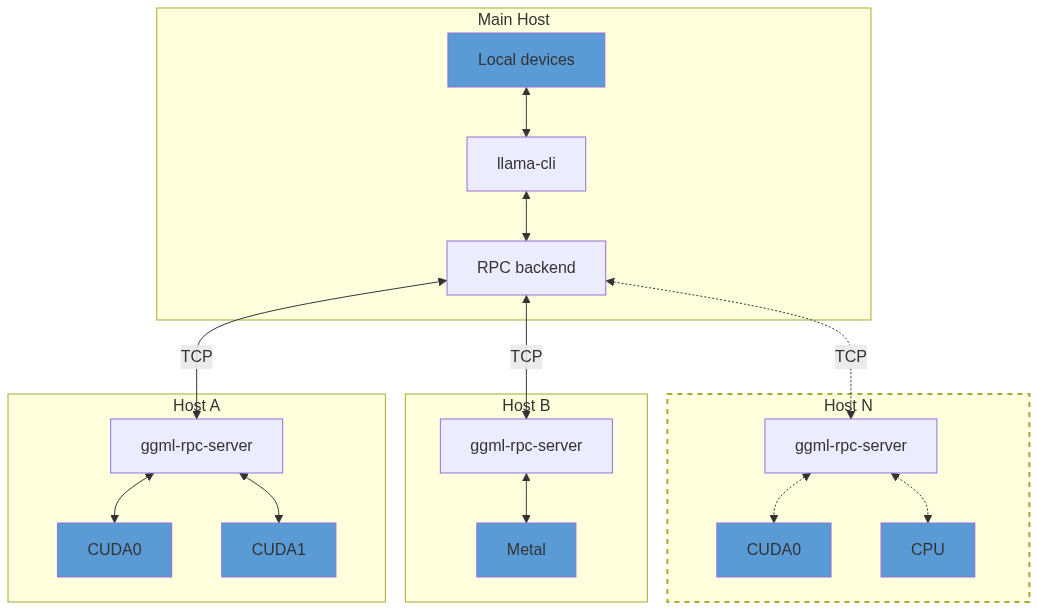
\includegraphics[width=0.78\textwidth]{figures/llamacpp_rpc_official.png}
\caption{Architecture of the \texttt{llama.cpp} RPC backend: the main host runs \texttt{llama-cli} (or \texttt{llama-bench}) with the RPC backend, which drives one \texttt{ggml-rpc-server} per remote host over TCP; each server exposes the local compute devices. Rendered from the Mermaid source in the official documentation (\texttt{tools/rpc/README.md} of~\cite{llamacpp}). In our cluster every host exposes its CPU, and the main host also runs a local RPC server.}
\label{fig:llamacpp-arch}
\end{figure}

\subsubsection{Distributed Llama}\label{sec:n2_3_2}
Distributed Llama~\cite{distributedllama} takes this idea further for clusters made of home or edge devices, and it uses a Root-Worker Architecture which includes \emph{root} node to load the model and tokenizer and send model slices to one or more \emph{worker} nodes over Ethernet, while the root node also calculates its own part so no device is left sitting idle, and this framework uses tensor parallelism where the root and worker nodes exchange partial activations after every layer to rebuild the full layer output before moving to the next layer, following the all-reduce pattern of Eq.~\ref{eq:allreduce}, which is exactly the per-token \texttt{Sync} step and the \texttt{Sent}/\texttt{Recv} network traffic we show in Section~\ref{sec:n8_2}--\ref{sec:n8_3}, but the framework has two architectural limits that directly decide our experiment setups, where the number of nodes must be a power of two like 1, 2, 4, 8 and so on, and it is also limited by the number of key-value attention heads in the model, which is why our baseline uses 1, 2, and 4 nodes, and going bigger would need either a larger node count that follows this rule or a model with more KV heads. Figure~\ref{fig:dllama-arch} summarizes the architecture.

\begin{figure}[H]
\centering
\begin{minipage}[c]{0.62\textwidth}\centering
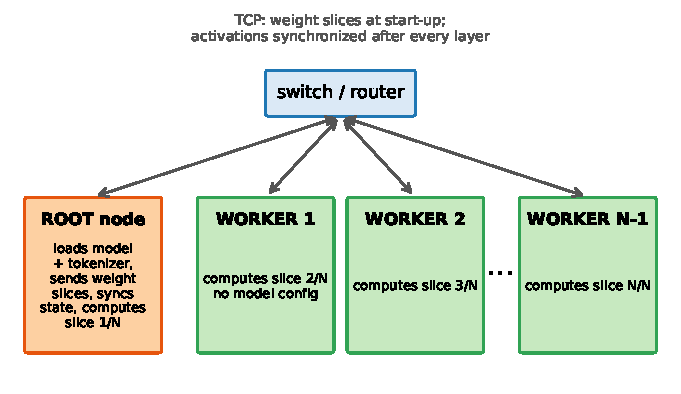
\includegraphics[width=\textwidth]{figures/dllama_architecture.pdf}
\end{minipage}\hfill
\begin{minipage}[c]{0.34\textwidth}\centering
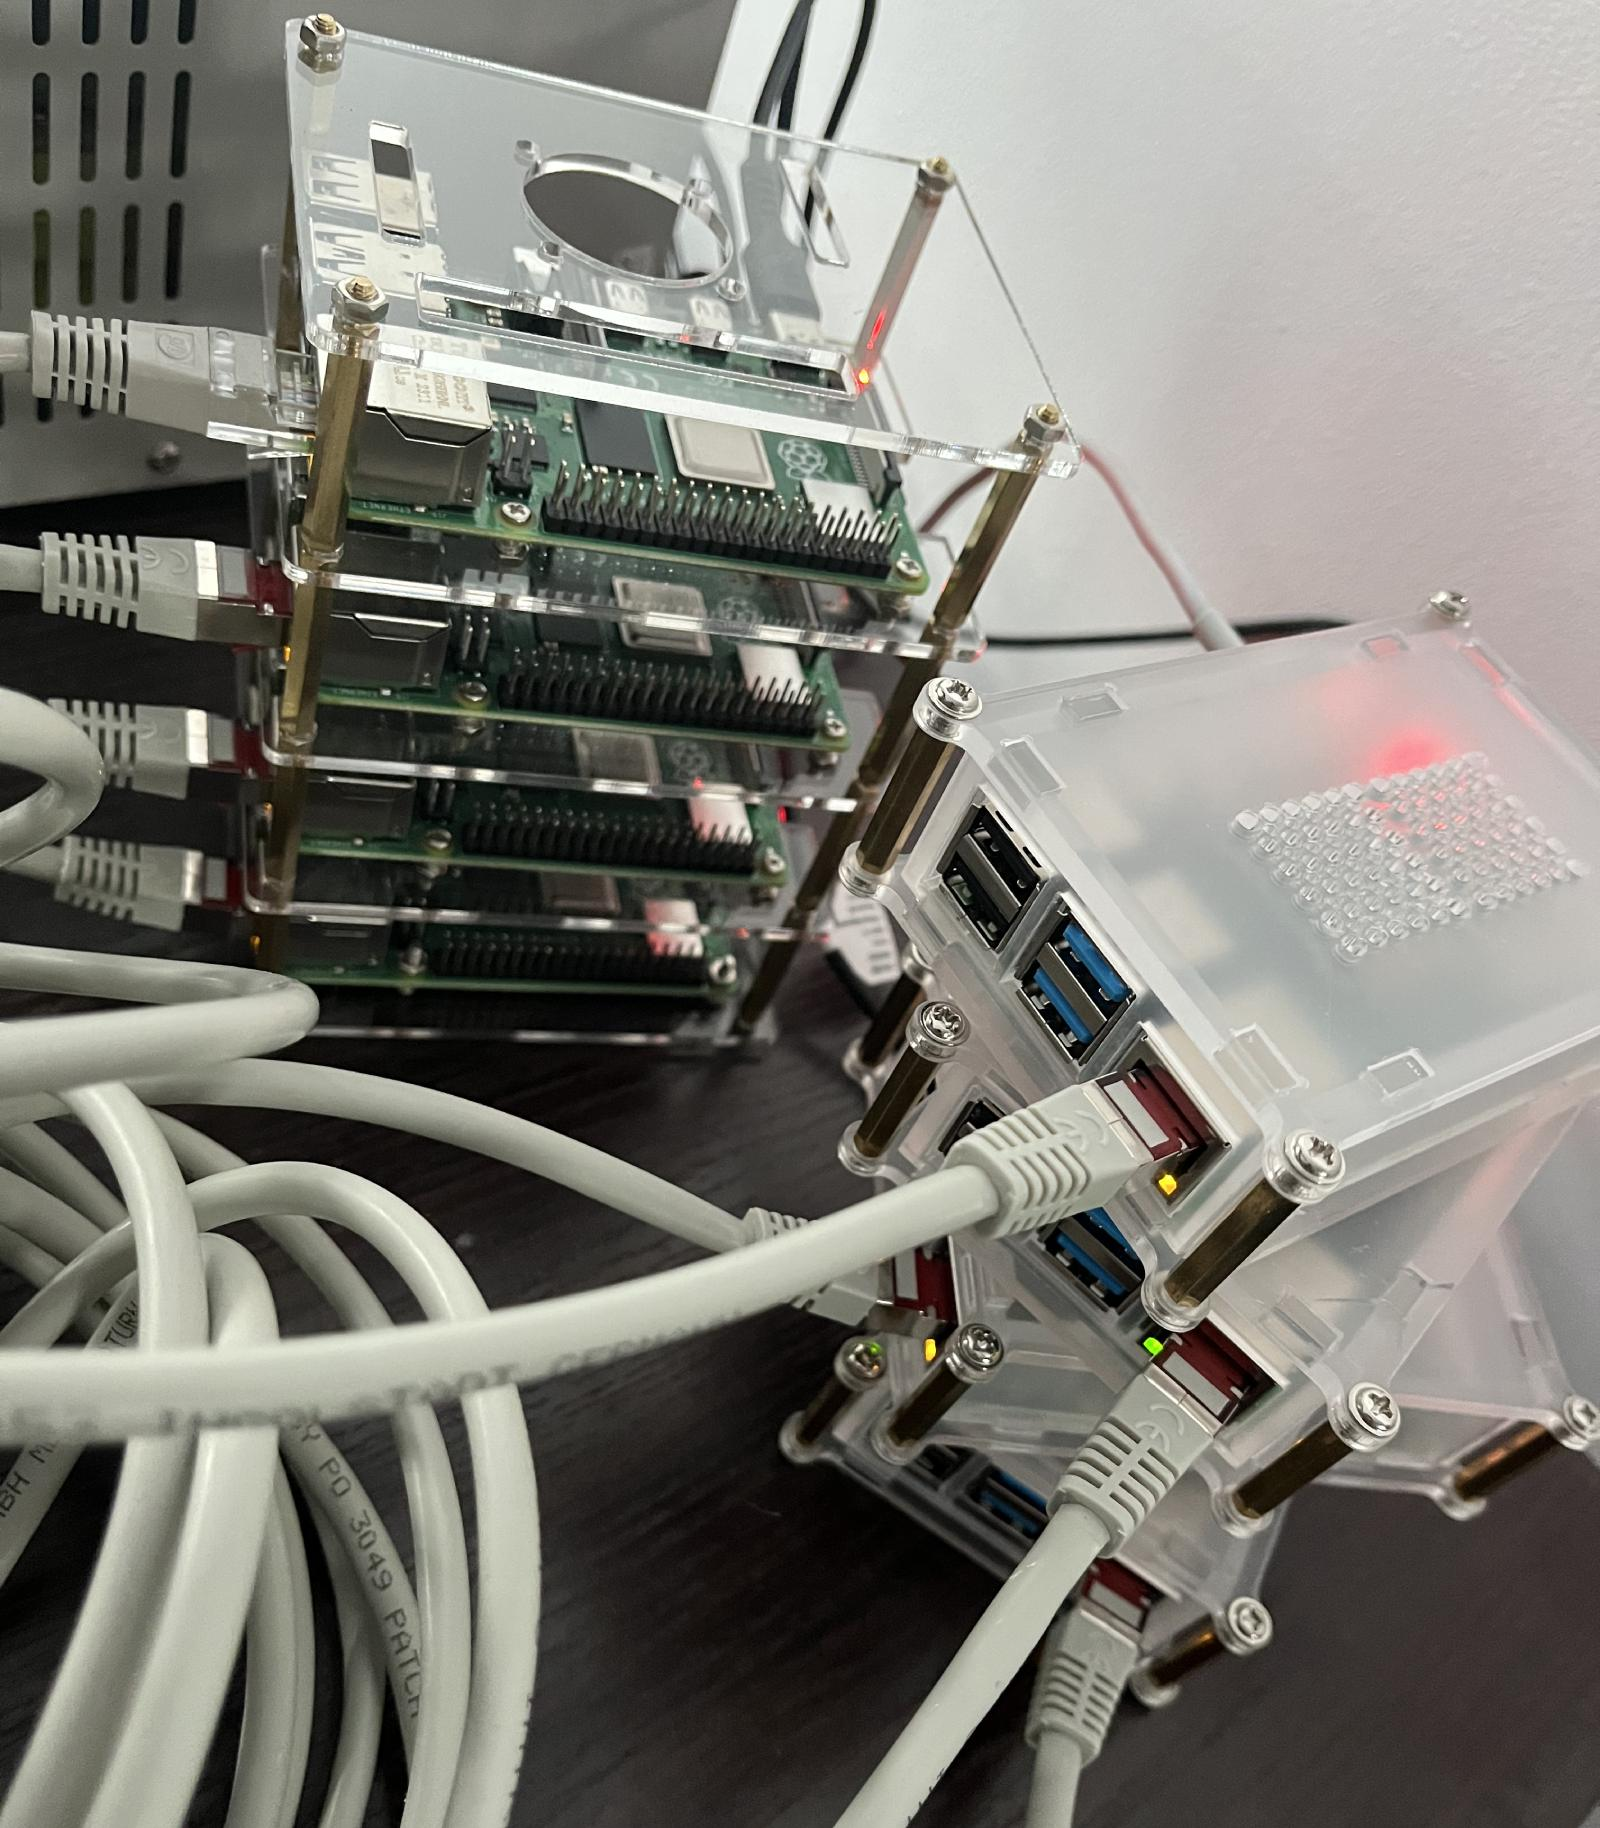
\includegraphics[width=\textwidth]{figures/dllama_8raspi_official.jpg}
\end{minipage}
\caption{Distributed Llama. Left: root/worker architecture, drawn by us from the architecture section of the official README~\cite{distributedllama} (the project provides no architecture figure). Right: the 8-Raspberry-Pi cluster shown in the official repository~\cite{distributedllama}.}
\label{fig:dllama-arch}
\end{figure}

\subsection{Quantization}\label{sec:n2_4}

By using Quantization, we can lower the numerical precision of model weights and sometimes activations, for memory-constrained devices usually changing 16-bit or 32-bit floats into 8-bit or 4-bit values. For a model with $P$ parameters quantized to $b$ bits per weight, the resulting memory footprint is approximately
\begin{equation}
M \approx \frac{P \cdot b}{8} \  \text{bytes}
\label{eq:quant-memory}
\end{equation}
before accounting for small per-block scale-factor overheads that quantization schemes such as Q4\_0 add on top of the raw bit width. This directly cuts down the memory size roughly linearly in $b$ and saves memory bandwidth when loading weights during inference (recall from Eq.~\ref{eq:intensity} that decode is bandwidth-bound, so halving $b$ roughly halves the bytes streamed per token), while only causing a very small and acceptable drop in generation quality. Llama-3.2-3B-Instruct has $P \approx 3.2 \times 10^{9}$ parameters, so Eq.~\ref{eq:quant-memory} with $b=4$ bits (Q4\_0) predicts $M \approx 1.6$~GB, which is close to the roughly 1.8~GB we observe once per-block scale factors and metadata are included; this still fits inside the 4~GB RAM of one Raspberry Pi node even before splitting across the cluster, but the larger Qwen-3-8B model ($P \approx 8 \times 10^{9}$) would need $M \approx 4$~GB by the same formula, in practice taking about 4--5~GB after Q4 quantization, which is the exact reason why we need to distribute it across multiple nodes.

% =====================================================
\section{Related Work}\label{sec:n3}

\subsection{Network Traffic Characteristics of Distributed Edge Inference}\label{sec:n3_1}
Buschmann et al.~\cite{buschmann2025} look into the network traffic generated by distributed LLM inference across edge devices to see how data patterns change with different parallel models and network setups. Their measurements characterize per-token traffic as a function of partitioning strategy and message size rather than treating throughput as the only outcome of interest, which mirrors the per-token \texttt{Sent}/\texttt{Recv} breakdown we use in Section~\ref{sec:n8_3} and gives us an external reference point for whether the growth predicted by Eq.~\ref{eq:allreduce} is actually realized on physical hardware. Their work is closely related to our RQ2 and RQ3 because they also treat network traffic as a primary metric rather than just focusing on throughput, but our study is different because we record network traffic together with sync latency and decode speed directly on real Raspberry Pi hardware, which lets us connect traffic growth directly to our sub-linear speedup in Section~\ref{sec:n8_2}--\ref{sec:n8_3} instead of just studying network traffic alone.

\subsection{Partitioning and Quantization on Heterogeneous Clusters}\label{sec:n3_2}
Zhao et al.~\cite{zhao2024} introduce LLM-PQ to run LLMs on heterogeneous setups using phase-aware partitioning and adaptive quantization, where each device is assigned a shard size and a bit width chosen so that the predicted per-device compute time under a cost model is balanced across the cluster, rather than splitting layers or tensors evenly as Distributed Llama does by default (Section~\ref{sec:n2_3_2}); this is conceptually the same load-balancing goal behind the speed-proportional splits we evaluate in Section~\ref{sec:n8_9}, except that we calibrate the split directly from measured single-device speeds rather than from an offline cost model. Zhang et al.~\cite{zhang2024edgeshard} build EdgeShard around a similar idea, using dynamic programming over profiled per-device latency and bandwidth to decide both the layer partition and the pipeline schedule, which shows that the partitioning problem in our setting can be posed as a constrained optimization over the same quantities we log (\texttt{Pred}, \texttt{Sync}, bytes sent/received) rather than solved purely by trial and error. Both works are directly relevant to our weighted splits and RQ4, because our goal of better model splitting shares the same basic idea of balancing workloads across boards, although we focus on homogeneous Raspberry Pi clusters with direct hardware tests instead of complex scheduling algorithms for heterogeneous nodes.

\subsection{Model Parallelism in Large-Scale Language Models}\label{sec:n3_3}
Shoeybi et al.~\cite{shoeybi2019} present Megatron-LM as a major milestone for using tensor parallelism to train huge language models across GPUs with NVLink, splitting attention heads and feed-forward matrices by row and column so that only two all-reduce operations of the form in Eq.~\ref{eq:allreduce} are needed per transformer layer; this established the basic synchronization design that both Distributed Llama and our experiments use. Their design implicitly assumes an Amdahl's-law-style scaling picture in which the fraction of time spent on communication, $p$, is small enough on high-bandwidth NVLink interconnects that the overall speedup with $N$ devices approaches
\begin{equation}
S(N) = \frac{1}{(1-p) + \dfrac{p}{N}}
\label{eq:amdahl}
\end{equation}
close to linear. Their work runs in data-center GPU clusters with interconnect bandwidth several orders of magnitude higher than our switched Gigabit Ethernet, so the communication fraction $p$ that Eq.~\ref{eq:amdahl} treats as negligible in their setting is, on our Raspberry Pi cluster, large enough to be the main term explaining the sub-linear speedups of 1.81$\times$ and 2.95$\times$ we measure in Section~\ref{sec:n8_2}. Comparing our measured sync overhead in Section~\ref{sec:n8_3} with their assumptions shows that edge setups are far more sensitive to network communication costs, and that Eq.~\ref{eq:amdahl} should really be extended with an $N$-dependent overhead term, $S(N) = \big[(1-p) + p/N + o(N)\big]^{-1}$, where $o(N)$ grows with the traffic predicted by Eq.~\ref{eq:allreduce}, to fit our data.

Besides network and model splitting, other works focus on reducing the actual computation during inference. Speculative decoding~\cite{leviathan2023fast} uses a small, cheap draft model to propose $\gamma$ candidate tokens, which the large target model then verifies in a single parallel forward pass; a proposed token is accepted with probability $\min\!\left(1, \frac{p_{\text{target}}(x)}{p_{\text{draft}}(x)}\right)$ under the target and draft distributions, and the expected number of tokens produced per target-model call is $\frac{1-\alpha^{\gamma+1}}{1-\alpha}$ for an average acceptance rate $\alpha$, so higher agreement between the two models directly multiplies decode throughput without changing the output distribution. KV cache methods~\cite{li2024surveykv} instead attack the memory-bandwidth bottleneck identified in Eq.~\ref{eq:intensity} directly, since the KV cache for a sequence of length $n$ occupies $2 \cdot n \cdot L \cdot d_{model} \cdot b/8$ bytes (factor 2 for keys and values, $L$ layers, $b$-bit storage), so techniques that prune, quantize, or evict cache entries reduce exactly the bytes that must be streamed per decode step in Section~\ref{sec:n2_1}. Both directions are largely orthogonal to our communication optimizations in Section~\ref{sec:n6_2}, so we treat them as interesting directions for future work in Section~\ref{sec:n9_3}.

\subsection{Positioning of This Work}\label{sec:n3_4}
Compared to these existing papers, our main contribution comes from direct empirical testing, because while simulation and GPU papers explain theoretical trade-offs, we provide real physical measurements on a cheap Raspberry Pi cluster that normal users or small labs can actually build, and our baseline results in Section~\ref{sec:n8_2}--\ref{sec:n8_3} clearly show sub-linear scaling caused by growing sync times and network traffic, consistent with the extended Amdahl-style model in Eq.~\ref{eq:amdahl}, which is a concrete finding that has not been directly reported for this exact setup in prior work.

% =====================================================
\section{Questions, Requirements and Metrics}\label{sec:n4}

\subsection{Research Questions}\label{sec:n4_1}

Based on the motivation in Section~\ref{sec:n1} and the background and related work in Sections~\ref{sec:n2}--\ref{sec:n3}, the core question we want to answer is: \emph{How does distributed LLM inference actually run on a cheap cluster of real Raspberry Pi boards, and what becomes the main bottleneck when we add more nodes?} And we break this down into four specific research questions:

\begin{itemize}
\item \textbf{RQ1.} How do decode throughput and time to first token scale when we use more Raspberry Pi nodes under the same model and quantization setting?
\item \textbf{RQ2.} How do pipeline parallelism and tensor parallelism compare in terms of latency, throughput, and network traffic on these low-cost devices?
\item \textbf{RQ3.} What is the main bottleneck here -- network bandwidth, latency, per-node memory bandwidth, or device count and heterogeneity -- and how does it change when the cluster grows larger?
\item \textbf{RQ4.} Can simple and low-effort optimizations, like better model splitting or reducing data transfer during sync, clearly improve throughput without hurting output quality too much?
\end{itemize}

\subsection{System Requirements}\label{sec:n4_2}

To answer these questions, our test setup needs to meet several basic requirements, where (R1) it has to support models that are too large for a single Raspberry Pi by spreading both memory and computation evenly across all available boards, and (R2) it should only use cheap commodity hardware like Raspberry Pi boards hooked up with a standard Gigabit Ethernet switch without any GPU or special high-speed network, while (R3) it must support any power-of-two total number of nodes without needing to manually re-slice the model every time, and (R4) it needs to record enough timing and network metrics for every generated token, such as compute time, sync time, and bytes transferred, so that we can clearly see what makes up the total latency, and finally (R5) the whole testing setup must be reproducible so we can run the same test again and get consistent results across different runs.

\subsection{Metrics of Experiment}\label{sec:n4_3}

Following these requirements, we track several key metrics that we use across all evaluations in Section~\ref{sec:n8}:

\begin{itemize}
\item \textbf{Time-to-first-token (TTFT)}: The total elapsed time from taking in a prompt to getting the very first token, which is mainly decided by the prefill phase discussed in Section~\ref{sec:n2_1},
\item \textbf{Decode throughput}: The average number of tokens generated per second during decoding, along with its inverse value which is the per-token latency in milliseconds,
\item \textbf{Network traffic}: How many kilobytes each node sends and receives for each generated token to show the actual communication cost,
\item \textbf{Synchronization time}: How much of the per-token latency is spent on waiting or doing inter-node sync instead of local compute, which corresponds to \texttt{Pred} and \texttt{Sync} in our logs,
\item \textbf{CPU and memory utilization}: The CPU load and RAM usage on each node during inference, so we can tell if a node is limited by compute, memory bandwidth, or just waiting on network packets, which is discussed in Section~\ref{sec:n8_5}.
\end{itemize}


% =====================================================
\section{Challenges and Possible Approaches}\label{sec:n5}

\subsection{Challenges of Edge Distributed Inference}\label{sec:n5_1}

\subsubsection{Memory and Compute Constraints}\label{sec:n5_1_1}
Each Raspberry Pi board in our cluster only has 4~GB of RAM and a basic ARM CPU without any dedicated matrix hardware, which directly limits how large a model slice each node can hold and how much compute power it can provide per token, so even when a model is partitioned well, the overall speed is still capped by the slowest node unless the workload is balanced very evenly across all devices.

\subsubsection{Network Communication Overhead}\label{sec:n5_1_2}
Splitting the workload introduces extra communication overhead that single-device setups do not have, and as shown by the Q4\_0-quantized 3B baseline in Section~\ref{sec:n8_3}, every extra node brings tens of kilobytes of traffic and tens of milliseconds of sync time for every single token, because the decode step generates tokens one by one and triggers network communication on every step instead of once per batch, so the communication latency directly limits the generation throughput, while a cheap Ethernet switch also cannot guarantee low and stable latency when handling multiple connections at once.

\subsubsection{Heterogeneity and Scalability of the Cluster}\label{sec:n5_1_3}
Real edge deployments mix devices of different performance levels. Our cluster contains two Raspberry Pi models with the same SoC and one board (RK3588) that is about 6.7$\times$ faster, so the slowest device can easily dictate the speed of the whole group. In addition, tensor parallelism in both frameworks requires the node count to be a power of two and is capped by the number of KV heads (8 for Llama-3.2-3B), so the cluster cannot grow one board at a time, and our seven Raspberry Pis can only form an 8-node tensor-parallel group together with the RK3588 board.

\subsection{Approaches and Design Alternatives}\label{sec:n5_2}

Facing these challenges, we looked at several possible options before deciding on our final approach in Section~\ref{sec:n6}. The first idea was to write a distributed inference system completely from scratch, but we decided not to do this because it would take too much time on basic engineering work rather than on testing and analysis, especially when frameworks like Distributed Llama and \texttt{llama.cpp} already have solid implementations of tensor and pipeline parallelism that fit our research questions. Another choice was to run everything inside a simulator like some related papers do in Section~\ref{sec:n3}, but we felt simulation alone could not show the real network delays from physical switches or the timing differences between real boards that RQ3 asks about, although we still used a laptop setup to do preliminary validation in Section~\ref{sec:n7_1} before testing on real hardware. So under our chosen tools, the main design question left is to choose between tensor and pipeline parallelism and pick the right splitting strategy for the two optimizations in RQ4, which we will explain in Section~\ref{sec:n6}.

% =====================================================
\section{Proposed Approach and Methodology}\label{sec:n6}

\subsection{Overview of Our Approach}\label{sec:n6_1}

Our work is mainly an empirical measurement study testing existing distributed inference methods, like tensor and pipeline parallelism from Distributed Llama and \texttt{llama.cpp}, on real physical edge hardware instead of proposing a brand-new parallel algorithm, and we choose this empirical approach because most related papers in Section~\ref{sec:n3} either use pure simulation or run on high-end hardware like data-center GPU clusters, so it is really unclear whether their findings about system bottlenecks and scaling rules still hold for cheap CPU-only setups with normal Ethernet, and verifying this on real boards is the main contribution we want to make.

\subsection{Experimental Methodology}\label{sec:n6_2}

Our overall method is divided into three clear stages:

\textbf{Stage 1 -- Baseline validation (completed, Section~\ref{sec:n8_2}--\ref{sec:n8_3}).} We start by running the default Distributed Llama framework directly on our test cluster using its original tensor-parallel mode across 1, 2, and 4 nodes for the Q4\_0-quantized Llama-3.2-3B-Instruct model, which sets up a solid baseline to compare with later tests and also confirms that our hardware, switch network, and software libraries are all working properly as reported in Section~\ref{sec:n8_2}--\ref{sec:n8_3}.

\textbf{Stage 2 -- Systematic exploration of the configuration space (completed, Section~\ref{sec:n8_4}--\ref{sec:n8_6}).} We switched to the RPC backend of \texttt{llama.cpp} so that tensor and pipeline parallelism (RQ2) can be compared with the same binaries, measured 1, 2, 4 and 8 nodes, and attributed the bottlenecks (RQ3) with two independent instruments: a resource monitor on every device (CPU, memory, network bytes and packets, sampled every 0.5~s) and a per-command timing log inside every RPC server. The comparison with Qwen-3-8B was dropped in favour of a deeper bottleneck analysis on one model.

\textbf{Stage 3 -- Optimization and evaluation (completed, Section~\ref{sec:n8_7}--\ref{sec:n8_9}).} The bottlenecks found in Stage~2 turned out to be different from the ones we expected in the mid-term plan: the per-token data volume is small and the network is not saturated, so lower-precision synchronization buffers would not help. Instead we implemented (i) a direct peer-to-peer allreduce that removes the head node from the synchronization path, (ii) an untied output layer that lets the largest matrix of the model be split across nodes, (iii) a switch that stops the head's RPC dispatcher threads from busy-spinning, which starved the head at 8 nodes, (iv) configuration-level optimizations (thread count, chunked pipelining, multi-request batching), and (v) speed-proportional (uneven) splits for a heterogeneous cluster, in the spirit of Zhao et al.~\cite{zhao2024} and Zhang et al.~\cite{zhang2024edgeshard}. Output quality is checked with perplexity for every change that could affect it (RQ4).

Across all three stages, we always keep the network topology fixed with a single switch in a star layout and use the same quantization level within each comparison set, changing only one variable at a time so that we can clearly see the impact of that specific change. All benchmark runs restart every RPC server first, report the mean of the repetitions of \texttt{llama-bench} (prompt of 32 tokens and 30 generated tokens unless stated otherwise), and record the temperature and throttling flags of every board. One Raspberry Pi 4B rebooted once because of an under-voltage during the 8-node experiments; after its power supply was replaced no board throttled, and the interrupted run was repeated.

% =====================================================
\section{Implementation}\label{sec:n7}

\subsection{Simulation and Validation}\label{sec:n7_1}

Before setting up the real Raspberry Pi boards, we first tested Distributed Llama and \texttt{llama.cpp} directly on a laptop using multiple local processes to simulate one root node and several workers talking through localhost, and this step let us check the whole build process, the model conversion flow that turns Hugging Face checkpoints~\cite{huggingface} into the quantized format needed by the framework, and the correctness of the final output tokens without worrying about the availability or stability of our physical boards.

\subsection{Hardware}\label{sec:hardware}

The final cluster has eight devices (Table~\ref{tab:hardware}): four Raspberry Pi~400 and three Raspberry Pi~4B boards, which share the Broadcom BCM2711 SoC (four Cortex-A72 cores at 1.8~GHz, 4~GB LPDDR4-3200, Gigabit Ethernet), and one LubanCat-5 board with a Rockchip RK3588 SoC (four Cortex-A76 cores at 2.3~GHz and four Cortex-A55 cores at 1.8~GHz, 4~GB). The Raspberry Pis run 64-bit Debian~13 and the LubanCat-5 runs Ubuntu~24.04. One Raspberry Pi~400 (rex) acts as the head: it holds the model file, runs the benchmark process and also one RPC server. Because nominal specifications say little about LLM inference, we measured the properties that matter (Table~\ref{tab:hardware}, Figure~\ref{fig:devperf}): the memory bandwidth with a small STREAM-style benchmark (copy and triad over 128~MB arrays, best of eight runs), the TCP throughput between two boards with a single stream, the round-trip time with \texttt{ping}, and the single-device decode and prefill speed with \texttt{llama-bench}.

\begin{table}[H]
\centering
\caption{Devices and their measured performance. Memory bandwidth: 4 threads (best single thread in parentheses). RTT is measured from the head (rex). Single-device speed: Llama-3.2-3B-Instruct Q4\_0, 4 threads, 32-token prompt. All devices have 4~GB RAM and Gigabit Ethernet; the measured TCP throughput between two devices is 940~Mbit/s.}
\label{tab:hardware}
\footnotesize
\begin{tabular}{@{}p{3.1cm}p{3.1cm}cccc@{}}
\toprule
Board (devices) & SoC / CPU & Mem.\ bandwidth & RTT & Prefill & Decode \\
\midrule
Raspberry Pi 400 (rex = head, finn, han, cassian) & BCM2711, 4$\times$A72 @ 1.8 GHz, LPDDR4-3200 & 3.7--4.2 GB/s (5.3) & 0.06--0.09 ms & 4.15 tok/s & 1.84 tok/s \\
Raspberry Pi 4B (luthen, jarjar, crosshair) & BCM2711, 4$\times$A72 @ 1.8 GHz, LPDDR4-3200 & 4.0--4.2 GB/s (5.3) & 0.07--0.09 ms & \multicolumn{2}{c}{same SoC as Pi 400} \\
LubanCat-5 (cat) & RK3588, 4$\times$A76 @ 2.3 GHz + 4$\times$A55 @ 1.8 GHz & 21--23 GB/s (21.6) & 0.24 ms & 48.75 tok/s & 12.28 tok/s \\
\bottomrule
\end{tabular}
\end{table}

\begin{figure}[H]
\centering
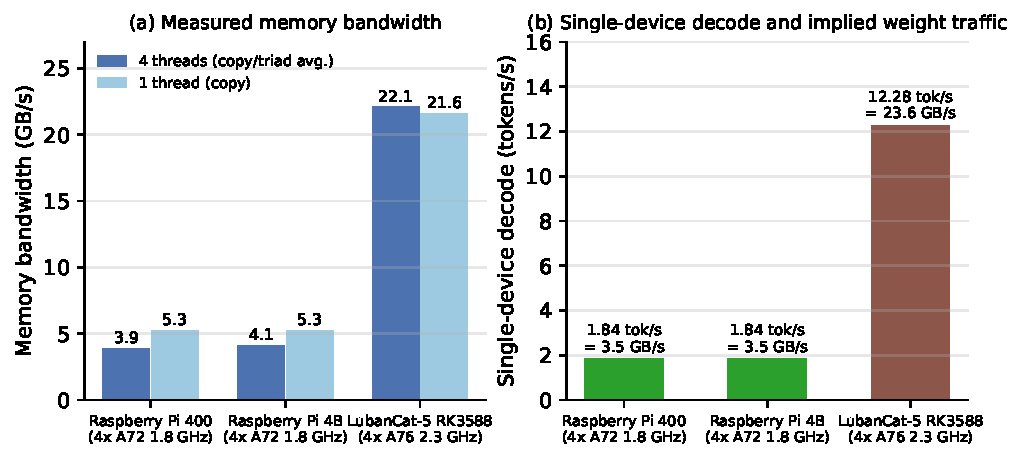
\includegraphics[width=0.95\textwidth]{figures/device_performance.pdf}
\caption{(a) Measured memory bandwidth. (b) Single-device decode speed; since every generated token reads the whole 1.92~GB of weights, the decode speed implies the memory traffic shown in the labels, which is close to the measured bandwidth of each device.}
\label{fig:devperf}
\end{figure}

\subsection{Network Topology and Communication}\label{sec:n7_3}

All nodes are connected through a single Gigabit Ethernet switch (a Netgear M4300-28G, used as a plain layer-2 switch plus a DHCP server) in a star topology: every device has a direct, single-hop link to the switch, and no device relays traffic for another (unlike a chain or ring topology).

\begin{figure}[H]
\centering
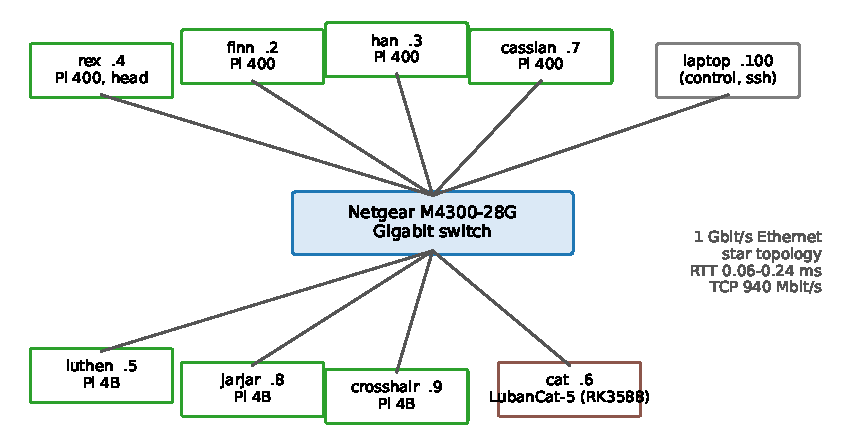
\includegraphics[width=0.8\textwidth]{figures/topology.pdf}
\caption{Topology of the final cluster: seven Raspberry Pi boards, one LubanCat-5 (RK3588) board and the controlling laptop, all connected to one Gigabit switch (last octet of the 10.77.0.0/24 address shown).}
\label{fig:topology}
\end{figure}

\begin{figure}[H]
\centering
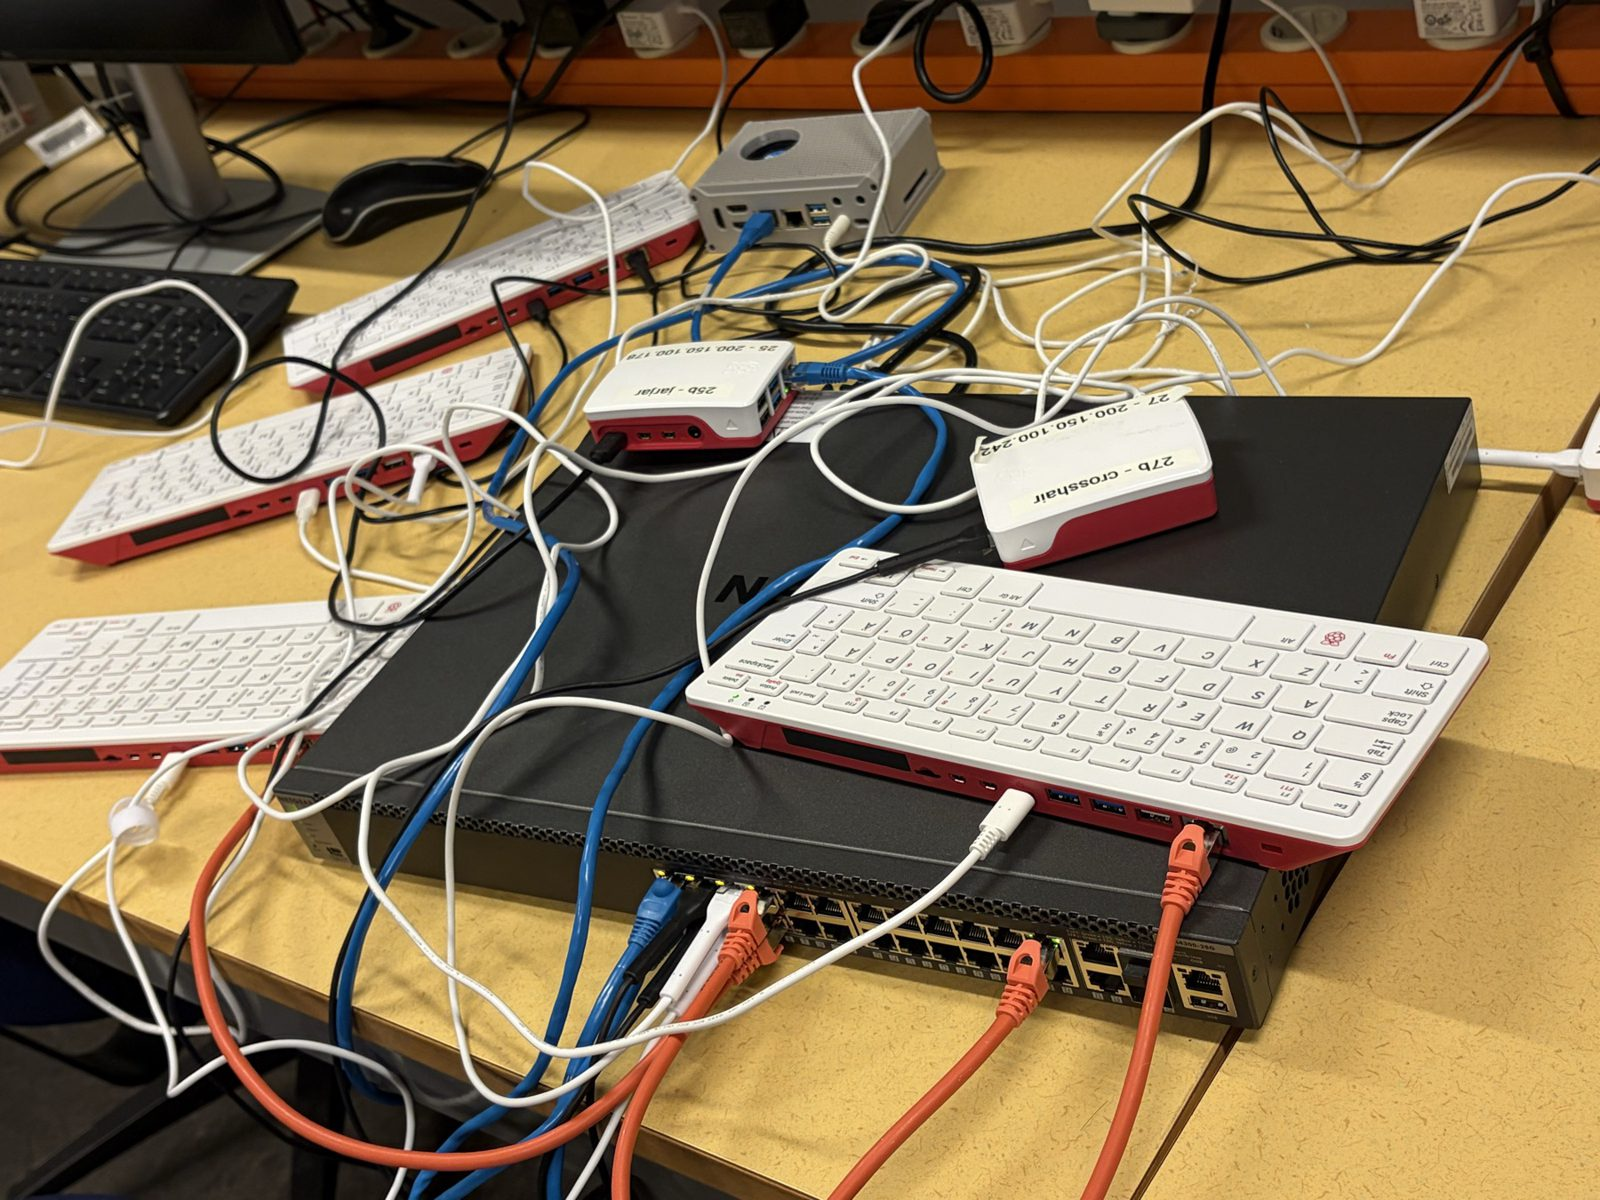
\includegraphics[width=0.75\textwidth]{figures/cluster_photo.jpg}
\caption{Our cluster in the lab: the Netgear M4300-28G switch (centre) with Raspberry Pi 400 keyboards, Raspberry Pi 4B boards in red-and-white cases (e.g.\ jarjar and crosshair, labelled) and the LubanCat-5 (RK3588) board in the grey case at the back.}
\label{fig:cluster-photo}
\end{figure}

We picked this layout because it directly matches the root-to-worker point-to-point communication pattern used in tensor parallelism in Section~\ref{sec:n2_3_2}, and it is also the easiest and cleanest way to separate compute latency from network delays.

\subsection{Deployment on the Pi Cluster}\label{sec:n7_4}

\subsubsection{Root/Head Node and Worker Roles}\label{sec:n7_4_1}
Following the design of Distributed Llama in Section~\ref{sec:n2_3_2}, one Raspberry Pi works as the root node to load the quantized model and tokenizer, process incoming prompts, run the generation loop, and send the model slices to all workers over the local network during startup, while the other boards just run the worker process listening on fixed IP addresses and ports, so they do not need any manual model configuration as long as they know their own IP and the root IP.

\subsubsection{Model Partitioning across Devices}\label{sec:n7_4_2}
Both frameworks cut the model weights automatically and evenly across all nodes for tensor parallelism as described in Section~\ref{sec:n2_2_3}. \texttt{llama.cpp} additionally accepts per-device proportions (\texttt{-ts}), which we use for the heterogeneous experiments in Section~\ref{sec:n8_9}.

\subsection{Benchmarking and Monitoring Pipeline}\label{sec:n7_5}

To collect our baseline numbers in Section~\ref{sec:n8_2}--\ref{sec:n8_3}, we run the built-in benchmark tool using \texttt{dllama inference}, which logs the local prediction time (\texttt{Pred}), the sync wait time (\texttt{Sync}), and the network bytes sent and received for every single token, while also giving the total prompt evaluation and generation throughput at the end, so this fully covers requirement R4 from Section~\ref{sec:n4_2} for recording latency and network traffic.

\subsection{Deployment with the \texttt{llama.cpp} RPC Backend}\label{sec:n7_6}

For the pipeline/tensor comparison and all optimizations we use the RPC backend of \texttt{llama.cpp}. Every board runs \texttt{ggml-rpc-server -H 0.0.0.0 -t $T$}, where $T$ is the number of compute threads, and the head runs \texttt{llama-bench}, \texttt{llama-batched-bench} or \texttt{llama-cli} with \texttt{--rpc} listing all servers (including its own) and \texttt{-sm layer} or \texttt{-sm tensor}. Only the head needs the model file; the workers receive their weight shards over the network at start-up. Binaries are cross-compiled on a laptop in an ARM64 Docker container (statically linked, \texttt{-mcpu=cortex-a72}) and distributed as release archives, so that a new board is ready in about one minute instead of compiling for tens of minutes on the Pi. All scripts (setup, health check, benchmark, trace analysis) and raw logs are kept in a public repository\footnote{\url{https://github.com/44sunsetsf/dat300-edge-llm}; the modified \texttt{llama.cpp} is the \texttt{dat300} branch of \url{https://github.com/44sunsetsf/llama.cpp}.}, together with a step-by-step guide that states on which machine each step runs.

\subsection{Per-Node Timing Log}\label{sec:trace}

To answer RQ3 we need to know where each token's time goes on every node, which neither \texttt{llama-bench} nor Distributed Llama's \texttt{Pred}/\texttt{Sync} summary reveals for \texttt{llama.cpp}. We added an optional timing log to the RPC server (enabled by the environment variable \texttt{GGML\_RPC\_TRACE}): for each command it records the start time, the idle time before the command, the duration, and details such as the number of bytes or graph nodes. For an allreduce it further splits the duration into waiting for the local computation, the network exchange (which includes waiting for the slowest peer) and the local summation. A script segments the log into tokens and reports, per node, the average time spent on computation, synchronization, data transfer and idling. With logging enabled, 2-node decode throughput changes from 2.93 to 2.90 tokens/s, i.e.\ the overhead is about 1\%.

\subsection{Resource Monitoring on Every Device}\label{sec:monitor}

To attribute the bottleneck from the resource side as well, every benchmark run starts a small monitor on each device. It is a single C process (statically compiled for ARM64, so it runs unchanged on the Raspberry Pis and on the RK3588) that every 0.5~s reads \texttt{/proc/stat} (user, system, idle and I/O-wait CPU time), \texttt{/proc/meminfo}, the resident memory of the RPC server and benchmark processes, the byte and packet counters of the Ethernet interface and the SoC temperature. The head runs the benchmark with \texttt{--progress} and timestamps every progress line, so that the samples can be split exactly into the prefill and decode phases, excluding model loading (when the head uploads about 2~GB of weights) and warm-up runs. Because the boards have no real-time clock and no internet access, their clocks drift and reset on reboot; the benchmark script therefore measures each device's clock offset relative to the laptop before each run and the analysis corrects all timestamps (offsets of 0.4--1.5~s were observed). For each device and phase the analysis reports CPU utilization, peak memory, network throughput, packet rate, and bytes and packets per generated token. A first version written as a shell script spawned several processes per sample and cost 5\% of decode throughput; the C version costs nothing measurable on 2 nodes (3.43--3.44 vs.\ 3.44 tokens/s) and 2--3\% on 4 nodes where all cores are busy (4.72--4.75 vs.\ 4.85 tokens/s).

\subsection{Modification 1: Direct Peer-to-Peer Allreduce}\label{sec:allreduce}

Stock \texttt{llama.cpp} (commit \texttt{bd4eeaa}) only lets the RPC servers exchange partial results directly when there are exactly two of them; for any other count the allreduce falls back to a generic path in which the head downloads every partial tensor, sums them and uploads the result again. We generalized the direct path to any power-of-two number of nodes up to 16 using \emph{recursive doubling}: in round $k$ each rank $r$ exchanges its current partial sum with rank $r \oplus 2^k$ and adds what it receives, so after $\log_2 N$ rounds every rank holds the full sum. Each rank therefore sends
\begin{equation}
V_{\text{rd}} = \log_2(N)\, d_{model}\, s
\label{eq:rd}
\end{equation}
bytes per allreduce, compared with $V_{\text{ag}} = (N-1)\, d_{model}\, s$ for an all-gather variant that finishes in a single round (also implemented and selectable with an environment variable). With $d_{model}=3072$ and $s=4$ bytes, one round moves 12~KB, so a 4-node token needs $56 \times 2 \times 12~\text{KB} \approx 1.4$~MB per node, in line with the 1.5--1.6~MB we measure (Table~\ref{tab:tp-scaling}). We also sum small payloads directly in host memory instead of building a separate compute graph for the addition (local summation time per token 3~ms $\rightarrow$ 0.9~ms), let all ranks build a full mesh of connections at start-up, and increased the listen backlog of the server socket from 1 to 64, which fixed a start-up deadlock when eight servers connect to each other simultaneously (found in an 8-container simulation on the laptop).

\subsection{Modification 2: Untied Output Layer}\label{sec:untied}

Llama-3.2 ties the output projection (\texttt{lm\_head}, $128256 \times 3072$, stored as Q6\_K, 323~MB, 18\% of the model file) to the input embedding: the GGUF file contains only \texttt{token\_embd.weight}, which is used both to look up the input token and to compute the logits. \texttt{llama.cpp}'s tensor-split rules split a tensor named \texttt{output.weight} along the vocabulary dimension, but treat \texttt{token\_embd.weight} as a replicated (``mirrored'') tensor, so when the model is tied every node computes the complete output projection. Our script \texttt{untie\_output.py} (using the \texttt{gguf} Python package) rewrites the model file with an additional \texttt{output.weight} tensor that is a byte-for-byte copy of \texttt{token\_embd.weight}. The arithmetic is unchanged, but the output layer is now split $N$ ways. The file grows from 1.92 to 2.25~GB, which only matters on the head.

\subsection{Modification 3: No Busy-Spinning in the Head's RPC Dispatchers}\label{sec:nospin}

The \texttt{llama.cpp} RPC client uses one dispatcher thread per remote device; while commands keep arriving, each dispatcher busy-spins on its queue instead of sleeping, to save the wake-up latency. With eight devices, the head (a 4-core Raspberry Pi) runs eight spinning dispatcher threads next to its own four-thread RPC server. Section~\ref{sec:n8_6} shows that this starves the threads that actually issue the work. We added an environment variable \texttt{GGML\_RPC\_NO\_SPIN} that makes the dispatchers block on their queues; our scripts set it by default.

\subsection{Network Configuration}\label{sec:n7_12}

Our first measurements on the switch were repeatedly interrupted because boards disappeared from the network for tens of seconds. The NetworkManager log on the boards showed the cause: the wired interfaces were configured for DHCP, the switch had no DHCP server, and after each 45-second DHCP timeout NetworkManager declared the connection failed and reset the interface, removing any manually added address. We enabled the switch's DHCP server with one static binding per board MAC address, gave the switch itself a management address, and additionally configured every board with the same static address, so that the cluster no longer depends on any DHCP server. Afterwards the network was stable (0\% packet loss, round-trip time 0.06--0.24~ms, Table~\ref{tab:hardware}). The subnet 10.77.0.0/24 was chosen because the laptops' Wi-Fi uses 10.0.0.0/16, which would otherwise shadow the cluster addresses.

\subsection{Builds for Heterogeneous Boards}\label{sec:n7_13}

The generic ARM64 build targets the Cortex-A72 of the Raspberry Pi, which lacks the \texttt{SDOT} dot-product instructions (\texttt{asimddp}) that \texttt{llama.cpp} uses for its Q4\_0 kernels on newer cores. For the RK3588 board we build the same commit with \texttt{-mcpu=cortex-a76}; the setup script detects the Cortex-A76 cores and installs this build automatically, and the benchmark script pins its RPC server to the four big cores. Since all builds come from the same commit, they interoperate in one cluster.

% =====================================================
\section{Evaluation}\label{sec:n8}

\subsection{Experimental Setup and Evaluation Goals}\label{sec:n8_1}
The evaluation has two parts. Sections~\ref{sec:n8_2}--\ref{sec:n8_3} report the baseline obtained with Distributed Llama on 1, 2 and 4 nodes. Sections~\ref{sec:n8_4}--\ref{sec:n8_9} report the \texttt{llama.cpp} experiments on 1--8 devices, measured in two lab sessions (four Raspberry Pis plus the RK3588 board on 2026-10-14, all eight devices on 2026-10-21), with the resource monitor and, where noted, the timing log. The main goal of the first test round is to make sure our cluster works reliably and get an unoptimized performance baseline before we start changing any code, so we run the official \texttt{dllama inference} benchmark on Distributed Llama~\cite{distributedllama} using the Q4\_0-quantized Llama-3.2-3B-Instruct model with its default tensor-parallel setup, and we only change the node count using 1, 2, and 4 Raspberry Pi boards while keeping the model, the quantization format, and the switch network completely the same, and for each run we track per-token numbers like prediction time (\texttt{Pred}), sync time (\texttt{Sync}), bytes sent and received per board, and the overall throughput values.

\subsection{Baseline: Scaling with the Number of Nodes}\label{sec:n8_2}
Table~\ref{tab:baseline} shows the baseline numbers we got on 1, 2, and 4 nodes, where each run generated 30 tokens after a warm-up phase of 32 prompt batches and 2 tokens.

\begin{table}[H]
\centering
\caption{Baseline results for Llama-3.2-3B-Instruct (Q4\_0) on 1, 2 and 4 Raspberry Pi nodes connected through a switch, using the unmodified Distributed Llama framework.}
\label{tab:baseline}
\resizebox{\textwidth}{!}{%
\begin{tabular}{@{}lccccc@{}}
\toprule
Nodes & Sent/token & Recv/token & Eval.\ tok/s (ms/tok) & Pred.\ tok/s (ms/tok) & Speedup (pred.) \\
\midrule
1 & 0 kB   & 0 kB   & 2.04 (491.32) & 1.97 (508.16) & 1.00$\times$ \\
2 & 190 kB & 429 kB & 3.50 (285.44) & 3.55 (281.46) & 1.81$\times$ \\
4 & 571 kB & 911 kB & 5.38 (185.87) & 5.81 (172.02) & 2.95$\times$ \\
\bottomrule
\end{tabular}}
\end{table}

On a single board without any network communication, the decode speed runs at 1.97 tokens/s, but when we distribute the model over 2 nodes with tensor parallelism, the throughput goes up to 3.55 tokens/s, and reaching 4 nodes brings it to 5.81 tokens/s, which gives a speedup of 1.81$\times$ on 2 nodes and 2.95$\times$ on 4 nodes compared to running on just one board, but this is still noticeably lower than the ideal linear speedup of 2$\times$ and 4$\times$, consistent with the extended Amdahl-style model of Eq.~\ref{eq:amdahl} in Section~\ref{sec:n3_3}.

\subsection{Network Traffic Patterns during Inference}\label{sec:n8_3}
The network data sent and received for each token increases clearly as we add more nodes, starting from 0~kB on 1 node to 190~kB sent and 429~kB received on 2 nodes, and reaching 571~kB sent and 911~kB received on 4 nodes, which follows the qualitative trend predicted by Eq.~\ref{eq:allreduce} in Section~\ref{sec:n2_2_3}, and at the same time the sync time (\texttt{Sync}) grows from 0~ms on 1 node to about 20--26~ms on 2 nodes and 38--45~ms on 4 nodes, even though the local computation time (\texttt{Pred}) drops from 490--550~ms down to 250--265~ms and 126--180~ms, which shows that while adding boards cuts down per-node compute time, it brings a heavy sync overhead that explains why our speedup in Table~\ref{tab:baseline} is sub-linear.

\subsection{Pipeline vs.\ Tensor Parallelism in \texttt{llama.cpp}, 1 to 8 Nodes}\label{sec:n8_4}

Sections~\ref{sec:n8_2}--\ref{sec:n8_3} used Distributed Llama, which only offers tensor parallelism. To compare the two strategies on equal terms we repeated the scaling experiment with the \texttt{llama.cpp} RPC backend on the same switch. The 1--4 node measurements use Raspberry Pi~400/4B boards only; the 8-node measurements necessarily include the RK3588 board (Section~\ref{sec:n5_1_3}). Table~\ref{tab:tp-scaling} and Figures~\ref{fig:decode-scaling}--\ref{fig:prefill-scaling} summarize the results. Each RPC server uses $T=3$ threads for 2-node tensor parallelism, $T=4$ for 4 and 8 nodes, and $T=4$ for pipeline parallelism, where only one board computes at a time.

\begin{table}[H]
\centering
\caption{Scaling of \texttt{llama.cpp} (Llama-3.2-3B-Instruct Q4\_0, 32-token prompt, 30 generated tokens). The 8-node configurations consist of 7 Raspberry Pis and the RK3588 board. ``Direct allreduce'', ``untied'' and ``no-spin'' are our modifications 1--3 (Sections~\ref{sec:allreduce}, \ref{sec:untied}, \ref{sec:nospin}); rows without ``no-spin'' use the default busy-spinning dispatchers.}
\label{tab:tp-scaling}
\resizebox{\textwidth}{!}{%
\begin{tabular}{@{}lcccccc@{}}
\toprule
 & \multicolumn{2}{c}{2 nodes} & \multicolumn{2}{c}{4 nodes} & \multicolumn{2}{c}{8 nodes} \\
\cmidrule(lr){2-3}\cmidrule(lr){4-5}\cmidrule(lr){6-7}
Configuration (single node: prefill 4.14, decode 1.84 tok/s) & Prefill & Decode & Prefill & Decode & Prefill & Decode \\
\midrule
PP & 4.12 & 1.88 & 4.01 & 1.84 & 4.06 & 2.00 \\
TP, stock & 5.93 & 2.86 & 5.77 & 1.03 & 3.15 & 0.41 \\
TP, direct allreduce (tied model) & 5.94 & 3.00 & 9.68 & 2.99 & 12.34 & 1.42 \\
TP, direct allreduce + untied & 5.98 & 3.45 & 12.57 & 5.04 & 13.39 & 1.62 \\
TP, direct allreduce + untied + no-spin & 5.98 & 3.46 & 12.57 & 5.02 & \textbf{16.24} & \textbf{6.34} \\
\bottomrule
\end{tabular}}
\end{table}

\begin{figure}[H]
\centering
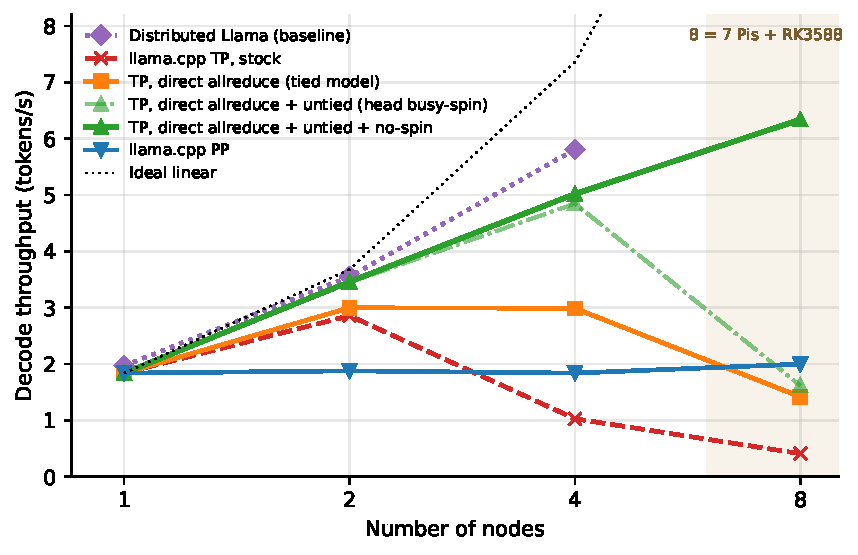
\includegraphics[width=0.8\textwidth]{figures/decode_scaling.pdf}
\caption{Decode throughput versus the number of nodes. The Distributed Llama curve is the baseline of Table~\ref{tab:baseline}. Stock \texttt{llama.cpp} TP collapses beyond 2 nodes. With our first two modifications TP scales to 4 nodes but collapses at 8 nodes because of the head's busy-spinning dispatchers; the third modification restores scaling to 6.34 tokens/s. PP stays at the single-node speed.}
\label{fig:decode-scaling}
\end{figure}

\begin{figure}[H]
\centering
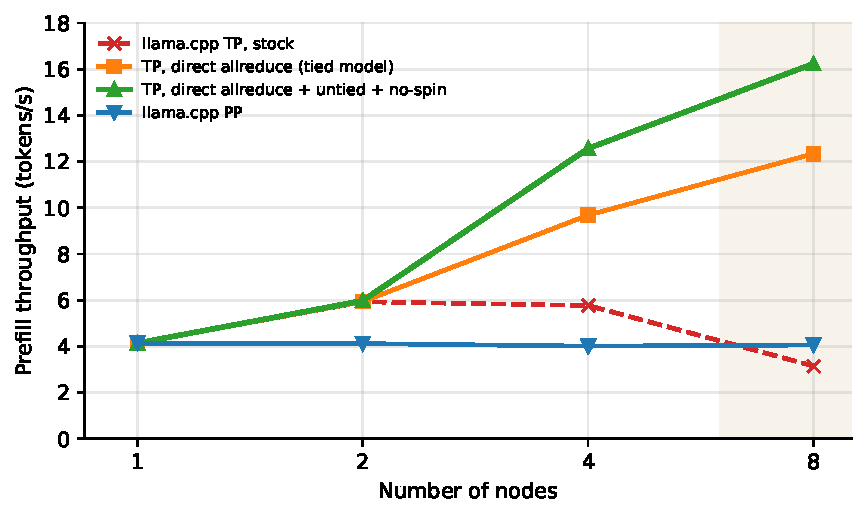
\includegraphics[width=0.78\textwidth]{figures/prefill_scaling.pdf}
\caption{Prefill throughput (32-token prompt) versus the number of nodes.}
\label{fig:prefill-scaling}
\end{figure}

These results answer RQ1 and RQ2. \emph{Pipeline parallelism never beats a single node for one request}: 1.84--2.00 tokens/s decode and 4.0--4.1 tokens/s prefill for 1--8 nodes, because the stages work strictly one after another (the small gain at 8 nodes comes from the RK3588 board computing its eighth of the layers faster). \emph{Stock tensor parallelism gets slower with more nodes} beyond two (0.41 tokens/s at 8 nodes). With all three modifications, tensor parallelism scales to 6.34 tokens/s decode (3.4$\times$ a single Raspberry Pi) and 16.24 tokens/s prefill (3.9$\times$) on 8 nodes. On 4 nodes it reaches 5.02--5.04 tokens/s, close to the Distributed Llama baseline (5.81 tokens/s prediction, 5.38 tokens/s evaluation), which uses its own TP implementation and model format.

\subsection{Resource Utilization}\label{sec:n8_5}

Table~\ref{tab:resources} and Figure~\ref{fig:resources} summarize the decode phase as seen by the resource monitor (Section~\ref{sec:monitor}). Four observations are important for attributing the bottlenecks.

\begin{table}[H]
\centering
\caption{Resource utilization in the decode phase (resource monitor, averages over the measured decode runs). CPU busy = 1 $-$ (idle + I/O wait). Memory is the resident memory of the RPC server (and of the benchmark process on the head). Network values are per worker Raspberry Pi (received + sent).}
\label{tab:resources}
\resizebox{\textwidth}{!}{%
\begin{tabular}{@{}lcccccccc@{}}
\toprule
Configuration & Decode & CPU head & CPU Pi workers & CPU RK3588 & Memory head / worker & Bytes / token & Packets / token & Link use \\
\midrule
Single node & 1.81 & 99.7\% & -- & -- & 2227 MB & -- & -- & -- \\
TP 2 & 3.44 & 75\% & 70\% & -- & 1349 / 956 MB & 1.67 MB & 1531 & 50 Mbit/s \\
TP 4, no-spin & 5.02 & 87\% & 79--83\% & -- & 887 / 494 MB & 2.76 MB & 2378 & 125 Mbit/s \\
TP 8, busy-spin & 1.62 & \textbf{94\%} & 15--17\% & 4\% & 665 / 262 MB & 4.3 MB & 3555 & 58 Mbit/s \\
TP 8, no-spin & 6.34 & 74\% & 61--65\% & 11\% & 671 / 262 MB & 3.9 MB & 3233 & 233 Mbit/s \\
PP 8 & 2.00 & 14\% & 10--14\% & 5\% & 630 / 181--235 MB & 30 kB & 48 & $<$1 Mbit/s \\
\bottomrule
\end{tabular}}
\end{table}

\begin{figure}[H]
\centering
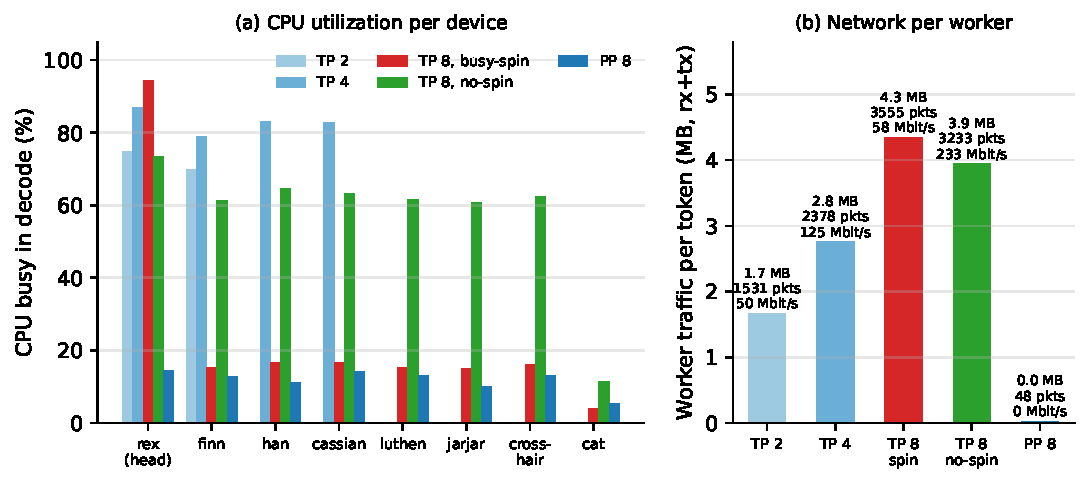
\includegraphics[width=0.98\textwidth]{figures/resources_decode.pdf}
\caption{(a) CPU utilization of every device in the decode phase. (b) Network traffic per generated token of a worker Raspberry Pi, with packets per token and average link utilization.}
\label{fig:resources}
\end{figure}

\emph{First}, a single Raspberry Pi keeps all four cores busy (99.7\%), and its decode speed of 1.84 tokens/s means reading the 1.92~GB of weights at 3.5~GB/s, which is 70--85\% of the measured memory bandwidth of 3.7--4.2~GB/s (Table~\ref{tab:hardware}). The RK3588 board's 12.28 tokens/s correspond to 23.6~GB/s, also its full bandwidth (Figure~\ref{fig:devperf}b). A single device is therefore memory-bandwidth bound, as predicted by Eq.~\ref{eq:intensity}.
\emph{Second}, the network is far from saturated: even at 8 nodes a worker transfers 3.9--4.3~MB per token, i.e.\ at most 233~Mbit/s of the 940~Mbit/s that a single TCP stream achieves. The bytes per token follow Eq.~\ref{eq:rd} closely: $2 \times 56 \times \log_2 N \times 12$~KB gives 1.4, 2.8 and 4.1~MB for 2, 4 and 8 nodes, compared with 1.7, 2.8 and 3.9--4.3~MB measured.
\emph{Third}, the 8-node runs with and without busy-spinning move \emph{the same} data per token (4.3 vs.\ 3.9~MB, 3555 vs.\ 3233 packets) but differ by 3.9$\times$ in speed, so the difference cannot come from the network; it coincides with the head's CPU being saturated (94\%) while the workers are idle 83--85\% of the time.
\emph{Fourth}, memory capacity is never limiting: the head needs at most 2.2~GB (single node) and a worker only $\approx$260~MB at 8 nodes, out of 3.4--3.6~GB available. Pipeline parallelism uses each board only $1/N$ of the time (10--14\% CPU) and transfers almost nothing (30~kB per token, plus about 0.5~MB of logits from the last stage to the head).

\subsection{Bottleneck Analysis: Bandwidth, Latency, Memory or Heterogeneity?}\label{sec:n8_6}

\paragraph{Bottleneck 1: allreduce relayed through the head.} Stock \texttt{llama.cpp} lets the RPC servers exchange partial sums directly only when there are exactly two of them. With four servers, every one of the 56 allreduces per token makes the head download the partial tensors of all servers, add them, and upload the results again: the head sends 49.9~MB and receives 4.4~MB per token (Figure~\ref{fig:head-traffic}), and 4-node decode drops to 1.03 tokens/s; at 8 nodes it is 0.41 tokens/s. This is a limitation of the implementation, not of tensor parallelism: Distributed Llama on the same hardware reaches 5.81 tokens/s on 4 nodes.

\begin{figure}[H]
\centering
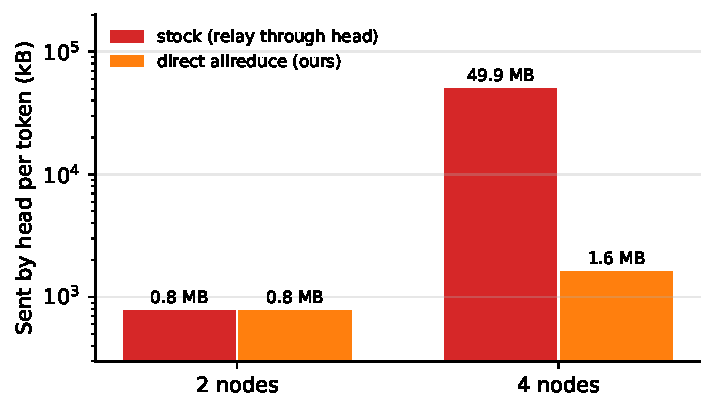
\includegraphics[width=0.58\textwidth]{figures/head_traffic.pdf}
\caption{Bytes sent by the head node per generated token (log scale). With four nodes the stock implementation relays every allreduce through the head.}
\label{fig:head-traffic}
\end{figure}

\paragraph{Bottleneck 2: the replicated output layer.} After removing bottleneck~1, 4-node decode (2.99 tokens/s) was no faster than 2-node decode (3.00 tokens/s). The timing log (Figure~\ref{fig:trace-breakdown}, Table~\ref{tab:trace}) shows that with the original model every node spends 80--85~ms per token on the final output projection, the same as with two nodes: the 323~MB output matrix is not split at all (Section~\ref{sec:untied}). In addition, the head computes each transformer layer almost twice as slowly as the workers (3.8 vs.\ 2.0~ms per layer), so the workers wait more than 100~ms per token inside the allreduce; this effect disappears completely with the untied model. With the untied output layer, the output projection takes 20--22~ms per node (one quarter), all nodes compute for the same time (131--141~ms), and a token takes 207~ms instead of 340~ms.

\begin{figure}[H]
\centering
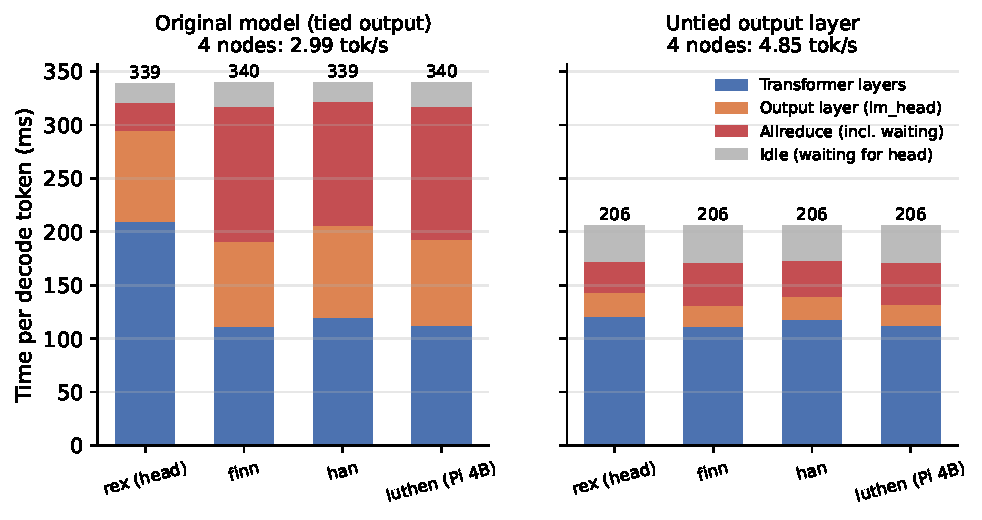
\includegraphics[width=0.95\textwidth]{figures/trace_breakdown_tp4.pdf}
\caption{Per-node decomposition of one decode token in 4-node TP, from the timing logs (average over 30 tokens). Left: original model; the output layer is computed in full on every node and the head is slow, so the workers wait in the allreduce. Right: untied output layer.}
\label{fig:trace-breakdown}
\end{figure}

\begin{table}[H]
\centering
\caption{Time per decode token from the timing logs (ms, average over 30 tokens). ``Allreduce'' includes waiting for the slowest peer; ``idle'' is time the server waits for the next command from the head.}
\label{tab:trace}
\resizebox{\textwidth}{!}{%
\begin{tabular}{@{}lllccccc@{}}
\toprule
Configuration & Model & Node & Layers & Output layer & Allreduce & Idle & Total \\
\midrule
4 nodes & Tied (original) & rex (head) & 209 & 85 & 26 & 18 & 339 \\
 & & Pi workers & 111--120 & 80--85 & 117--126 & 17--23 & 339--340 \\
4 nodes & Untied & rex (head) & 121 & 22 & 30 & 34 & 206 \\
 & & Pi workers & 111--118 & 20--21 & 33--40 & 33--35 & 206 \\
\midrule
8 nodes, busy-spin & Untied & rex (head) & 97 & 14 & 57 & \textbf{460} & 631 \\
 & & Pi workers & 64--72 & 10--11 & 76--86 & \textbf{469--472} & 631 \\
 & & RK3588 & 33 & 5 & 117 & \textbf{475} & 631 \\
8 nodes, no-spin & Untied & rex (head) & 81 & 12 & 47 & 14 & 154 \\
 & & Pi workers & 61--69 & 10--11 & 59--67 & 14--16 & 155 \\
 & & RK3588 & 21 & 3 & 107 & 23 & 155 \\
\bottomrule
\end{tabular}}
\end{table}

\paragraph{Bottleneck 3: the head's CPU at 8 nodes.} With modifications 1 and 2, decode scales from 3.45 (2 nodes) to 5.04 tokens/s (4 nodes) but falls to 1.62 tokens/s on 8 nodes, while prefill still increases (13.39 tokens/s). The resource monitor shows the head's CPU at 94\% during decode and the workers at 15--17\% (Figure~\ref{fig:cpu-timeline}, left), and the timing log shows every server idle for 460--475~ms of each 631~ms token, waiting for the head's next command (Figure~\ref{fig:trace8}, left). To find what the head spends its CPU on, we sampled the call stacks of the benchmark process with \texttt{gdb} fifteen times during decoding: the per-device dispatcher threads (Section~\ref{sec:nospin}) appear in almost every sample, each using 18--27\% of a core according to \texttt{top}. With eight devices, eight busy-spinning dispatchers plus the head's own four-thread RPC server compete for four cores, so the threads that do useful work only run intermittently.

We tested this explanation with four controlled variations (Figure~\ref{fig:head}). Reducing the benchmark process to one thread or the head's RPC server to two threads does not help (1.63 tokens/s), because the spinning threads still fill the cores. Moving the head role to the RK3588 board helps at 4 nodes (5.31 vs.\ 4.72 tokens/s) but is much worse at 8 nodes (0.72 tokens/s, idle time 1225~ms per token), because we pinned the benchmark process to the four slow Cortex-A55 cores, where the eight spinning dispatchers fight over even less CPU. Disabling the busy-spin (\texttt{GGML\_RPC\_NO\_SPIN=1}) on the original head raises 8-node decode from 1.62 to \textbf{6.34 tokens/s} and prefill from 13.39 to 16.24 tokens/s: the idle time drops from 470 to 15~ms per token, the workers' CPU rises from 15\% to 61--65\%, and the head's CPU falls to 74\% (Figure~\ref{fig:cpu-timeline}, right). On 4 nodes the same change gives +6\% (4.72 $\rightarrow$ 5.02 tokens/s) and on 2 nodes nothing (3.44 $\rightarrow$ 3.46 tokens/s), consistent with the number of spinning threads relative to the head's four cores.

\begin{figure}[H]
\centering
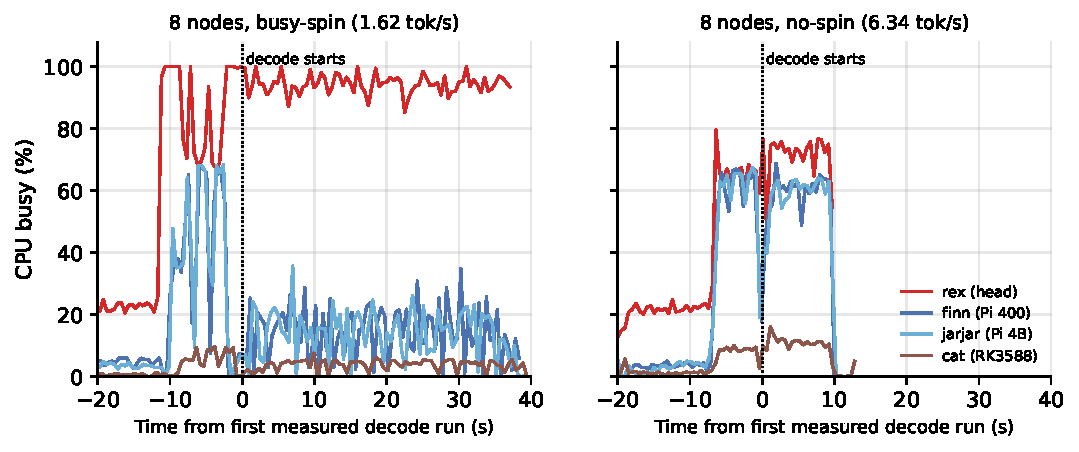
\includegraphics[width=0.98\textwidth]{figures/cpu_timeline_tp8.pdf}
\caption{CPU utilization over time in the 8-node TP runs (resource monitor, 0.5~s samples), aligned to the start of the first measured decode run. Left: default busy-spinning dispatchers; the head is saturated and the workers idle. Right: \texttt{GGML\_RPC\_NO\_SPIN=1}; all Raspberry Pis compute at 60--75\% and the run finishes four times sooner.}
\label{fig:cpu-timeline}
\end{figure}

\begin{figure}[H]
\centering
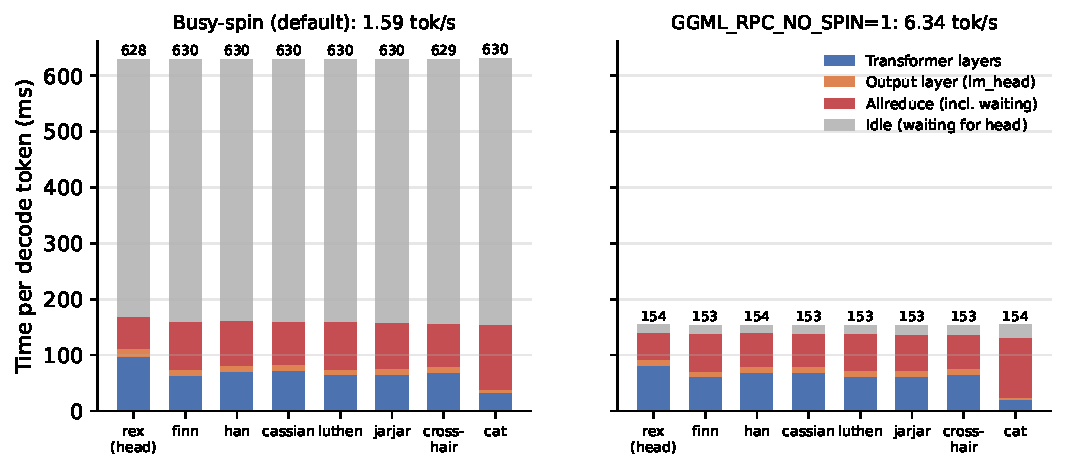
\includegraphics[width=0.98\textwidth]{figures/trace_breakdown_tp8.pdf}
\caption{Per-node decomposition of one decode token in 8-node TP (timing logs). With busy-spinning dispatchers (left) every node waits about 470~ms per token for the head; without (right) the idle time is 14--23~ms.}
\label{fig:trace8}
\end{figure}

\begin{figure}[H]
\centering
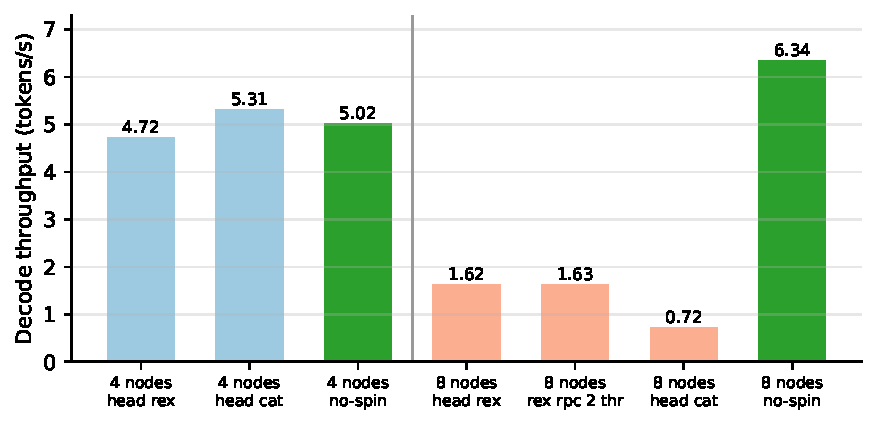
\includegraphics[width=0.72\textwidth]{figures/head_bottleneck.pdf}
\caption{Experiments on the head bottleneck (decode throughput, untied model).}
\label{fig:head}
\end{figure}

\paragraph{The network is not the bottleneck.} Bandwidth utilization is at most 25\% of the link (Table~\ref{tab:resources}), and the bytes and packets per token do not depend on whether the head busy-spins, while the speed changes by 3.9$\times$. The latency component is also small: at 8 nodes, 56 allreduces with $\log_2 8 = 3$ rounds each at a round-trip time of about 0.1~ms add roughly 17~ms per token. Halving the number of rounds with the all-gather algorithm (Eq.~\ref{eq:rd}) does not change the throughput on 4 nodes (4.81 vs.\ 4.85 tokens/s) or 8 nodes (1.56 vs.\ 1.62 tokens/s, with busy-spinning). The RK3588 board, which computes its share four times faster than the Raspberry Pis, spends the most time in the allreduce (107--117~ms): it waits for the slowest Raspberry Pi, which is how heterogeneity shows up in an even split.

\paragraph{A performance model.} The timing logs suggest the following model of the decode time per token on $N$ nodes:
\begin{equation}
T(N) = \frac{T_{L}}{N} + \frac{T_{O}}{k(N)} + n_{s}\, r(N)\, t_{r} + T_{h}(N),
\qquad k(N) = \begin{cases} 1 & \text{tied output} \\ N & \text{untied output} \end{cases}
\label{eq:model}
\end{equation}
where $T_L$ is the single-node time of the transformer layers, $T_O$ the single-node time of the output layer, $n_s = 56$ the number of allreduces per token, $r(N)=\log_2 N$ the number of rounds per allreduce, $t_r$ the time per round including waiting for the slowest peer, and $T_h(N)$ the time the servers wait for the head (sampling, fetching the logits, issuing the next commands). From the single-node throughput, $T_L + T_O = 1000/1.84 = 543$~ms, and the trace gives $T_O \approx 83$~ms, so $T_L \approx 460$~ms. With $t_r \approx 0.3$~ms and the measured $T_h = 8$, 33 and 15~ms for 2, 4 and 8 nodes, Eq.~\ref{eq:model} predicts 3.37, 4.94 and 7.5 tokens/s for the untied model (measured with no-spin: 3.46, 5.02 and 6.34; Figure~\ref{fig:perf-model}). At 8 nodes the measured allreduce time (59--67~ms) and the Raspberry Pis' layer time (61--69~ms instead of $460/8 = 58$~ms) are slightly larger than modelled. Before the no-spin change, $T_h(8)$ was 460~ms, which is why our mid-way projection of about 6~tokens/s for 8 nodes initially failed. The model also shows what limits further scaling: the compute terms shrink with $N$, while the synchronization term grows with $\log_2 N$ and $T_h$ does not shrink; at 8 nodes about half of each token is already spent outside computation, in line with Amdahl's law (Eq.~\ref{eq:amdahl}).

\begin{figure}[H]
\centering
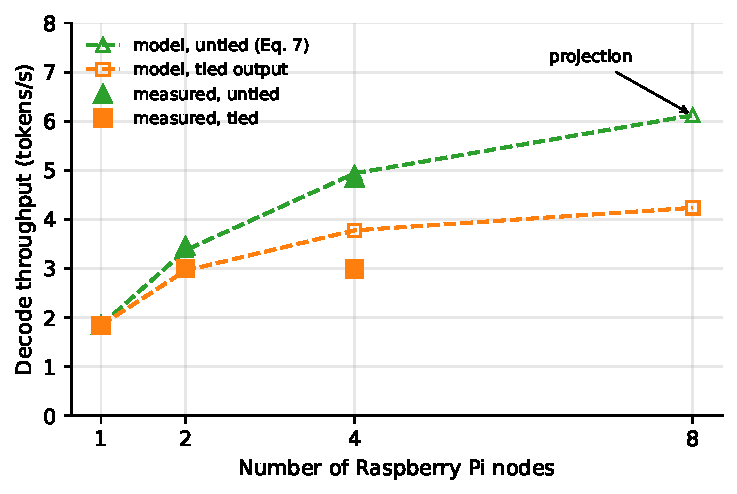
\includegraphics[width=0.64\textwidth]{figures/perf_model.pdf}
\caption{Decode throughput predicted by Eq.~\ref{eq:model} (dashed) and measured (markers).}
\label{fig:perf-model}
\end{figure}

\paragraph{Answer to RQ3.} On one board the bottleneck is memory bandwidth (decode reads the weights at 70--85\% of the measured bandwidth). On the cluster it moves to the parts of the system that do not shrink with $N$: in stock \texttt{llama.cpp} the head relaying all synchronization traffic, then the unsplit tied output layer, and at 8 nodes the head's CPU, which busy-spinning dispatcher threads exhaust. Network bandwidth is never the bottleneck (at most 25\% link utilization), network latency is a minor term ($\approx$10\% of a token), and memory capacity is not limiting for this model. Heterogeneity matters as soon as devices of different speed share an even split (Section~\ref{sec:n8_9}).

\subsection{Evaluation of Optimization Strategies}\label{sec:n8_7}

\subsubsection{Effect of Each Modification}\label{sec:n8_7_1}

Table~\ref{tab:ablation} and Figure~\ref{fig:ablation} show the effect of each optimization on 4 and 8 nodes. On 4 nodes the two main optimizations are complementary: the untied model alone does not help the stock implementation (1.03 $\rightarrow$ 1.09 tokens/s), because the head relay dominates, and the direct allreduce alone stops at 2.99 tokens/s, because the output layer is replicated; together they give 4.85 tokens/s, and 5.04 tokens/s with four threads per server. On 8 nodes the third modification is decisive (1.62 $\rightarrow$ 6.34 tokens/s); in total, 8-node decode improves 15.5$\times$ over stock \texttt{llama.cpp} (0.41 tokens/s). The improvement holds for long generations: with a 512-token prompt and 128 generated tokens, 4-node decode is 4.93 tokens/s with the untied model and 2.93 tokens/s with the original model.

\begin{figure}[H]
\centering
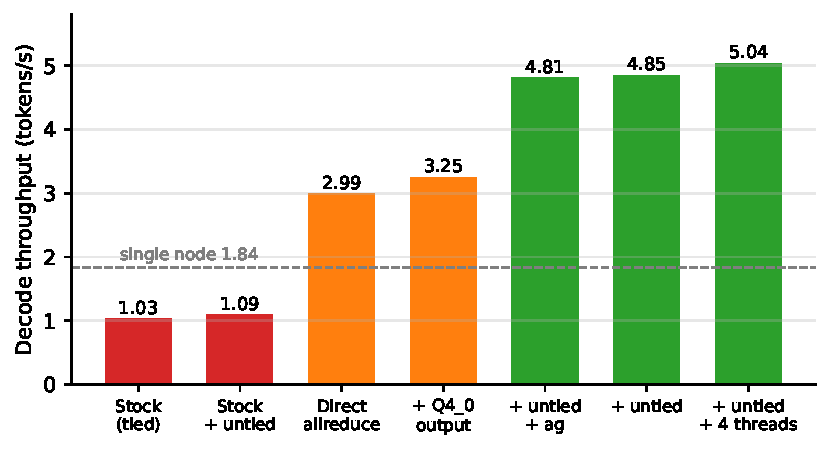
\includegraphics[width=0.76\textwidth]{figures/ablation_tp4.pdf}
\caption{Effect of each optimization on 4-node TP decode throughput.}
\label{fig:ablation}
\end{figure}

\begin{table}[H]
\centering
\caption{Ablation on 4 nodes (Raspberry Pis, 3 threads per server unless noted) and on 8 nodes (7 Raspberry Pis + RK3588, 4 threads).}
\label{tab:ablation}
\resizebox{\textwidth}{!}{%
\begin{tabular}{@{}llccc@{}}
\toprule
Nodes & Configuration & Prefill (tok/s) & Decode (tok/s) & vs.\ stock \\
\midrule
4 & Stock, original model & 5.77 & 1.03 & 1.0$\times$ \\
4 & Stock, untied model & 5.83 & 1.09 & 1.1$\times$ \\
4 & Direct allreduce, original model & 9.68 & 2.99 & 2.9$\times$ \\
4 & Direct allreduce, output layer re-quantized to Q4\_0 (tied) & 9.78 & 3.25 & 3.2$\times$ \\
4 & Direct allreduce, untied, all-gather allreduce & 10.01 & 4.81 & 4.7$\times$ \\
4 & Direct allreduce, untied & 10.07 & 4.85 & 4.7$\times$ \\
4 & Direct allreduce, untied, 4 threads & \textbf{12.57} & \textbf{5.04} & \textbf{4.9$\times$} \\
\midrule
8 & Stock, untied model & 3.15 & 0.41 & 1.0$\times$ \\
8 & Direct allreduce, original model & 12.34 & 1.42 & 3.5$\times$ \\
8 & Direct allreduce, untied & 13.39 & 1.62 & 4.0$\times$ \\
8 & Direct allreduce, untied, all-gather allreduce & 13.44 & 1.56 & 3.8$\times$ \\
8 & Direct allreduce, untied, no-spin & \textbf{16.24} & \textbf{6.34} & \textbf{15.5$\times$} \\
\bottomrule
\end{tabular}}
\end{table}

\subsubsection{Quantization and Communication Reduction}\label{sec:n8_7_2}

The mid-term plan proposed to reduce the synchronization volume with lower-precision buffers, i.e.\ to shrink $s$ in Eq.~\ref{eq:allreduce}. The resource measurements show that this would not pay off: link utilization is at most 25\%, and halving the number of synchronization rounds (all-gather) had no measurable effect. We therefore did not pursue it. Reducing the precision of the output layer instead (re-quantizing the tied embedding from Q6\_K to Q4\_0, all other tensors unchanged) makes the replicated output layer cheaper (+9\% on 2 nodes, 3.25 vs.\ 2.99 tokens/s on 4 nodes), but splitting the output layer (untying) is much more effective and does not change the model.

\subsubsection{Throughput--Accuracy Trade-off}\label{sec:n8_7_3}

Table~\ref{tab:ppl} checks the output quality. The untied model produces exactly the same perplexity as the original model in every chunk, as expected from an identical computation, and disabling busy-spinning only changes thread scheduling. Re-quantizing the output layer to Q4\_0 costs 0.6\% in perplexity, within the statistical uncertainty. Tensor parallelism itself changes the perplexity only in the last digits, because the prefill phase exchanges large tensors in BF16 (an upstream design choice) and the summation order differs. The best configuration therefore has no accuracy cost.

\begin{table}[H]
\centering
\caption{Perplexity checks (lower is better). Rows in the same group use the same evaluation text.}
\label{tab:ppl}
\resizebox{\textwidth}{!}{%
\begin{tabular}{@{}lll@{}}
\toprule
Model / configuration & Setting & Perplexity \\
\midrule
Original model, single node & 12 chunks of 256 tokens, RK3588 & 7.2208 $\pm$ 0.538 \\
Untied model, single node & same & 7.2208 $\pm$ 0.538 (identical in every chunk) \\
\midrule
Original model, single node & 6 chunks of 256 tokens & 8.08 \\
Output layer re-quantized to Q4\_0 & same & 8.13 (+0.6\%, within $\pm$0.27) \\
\midrule
Single node & 6 chunks, laptop simulation & 11.13 \\
Direct-allreduce TP, 4 / 8 nodes & same & 11.09 / 11.12 \\
\bottomrule
\end{tabular}}
\end{table}

\subsection{The Direct Allreduce under Limited Bandwidth (10~Mbit/s)}\label{sec:10mbps}

On a Gigabit switch the network is far from saturated, so the benefit of the direct allreduce over the stock relay mostly comes from removing the head's serial round trips. To see how much the change matters on a slow network, we repeated the 8-node comparison with every device's link limited to 10~Mbit/s. The devices' Ethernet interfaces were set to advertise only 10~Mbit/s full duplex (\texttt{ethtool -s eth0 advertise 0x002}), so that the corresponding switch ports also run at 10~Mbit/s; the laptop's port stayed at 1~Gbit/s for control. Because loading the weights over 10~Mbit/s would take about 8 minutes per run (the RPC servers' local cache does not cover the small tensor-parallel shards), the links are switched to 10~Mbit/s automatically right after the model is loaded, when the head reports the warm-up generation run, and switched back afterwards (\texttt{scripts/exp/bw\_limit.sh}). Only decode is measured, with the resource monitor running.

\begin{table}[H]
\centering
\caption{8-node tensor parallelism (7 Raspberry Pis + RK3588, untied model) at 1~Gbit/s and 10~Mbit/s links. Traffic is received + sent per generated token in the decode phase (resource monitor).}
\label{tab:10mbps}
\resizebox{\textwidth}{!}{%
\begin{tabular}{@{}lcccc@{}}
\toprule
Configuration & Link speed & Decode (tok/s) & Head traffic / token & Worker traffic / token \\
\midrule
Stock \texttt{llama.cpp} & 1 Gbit/s & 0.41 & -- & -- \\
Ours (direct allreduce + no-spin) & 1 Gbit/s & 6.34 (15$\times$) & 5.0 MB & 3.9 MB \\
Stock \texttt{llama.cpp} & 10 Mbit/s & 0.01 & 200.7 MB & 28.6 MB \\
Ours (direct allreduce + no-spin) & 10 Mbit/s & 0.20--0.26 (20--26$\times$) & 5.3 MB & 4.4 MB \\
\bottomrule
\end{tabular}}
\end{table}

\begin{figure}[H]
\centering
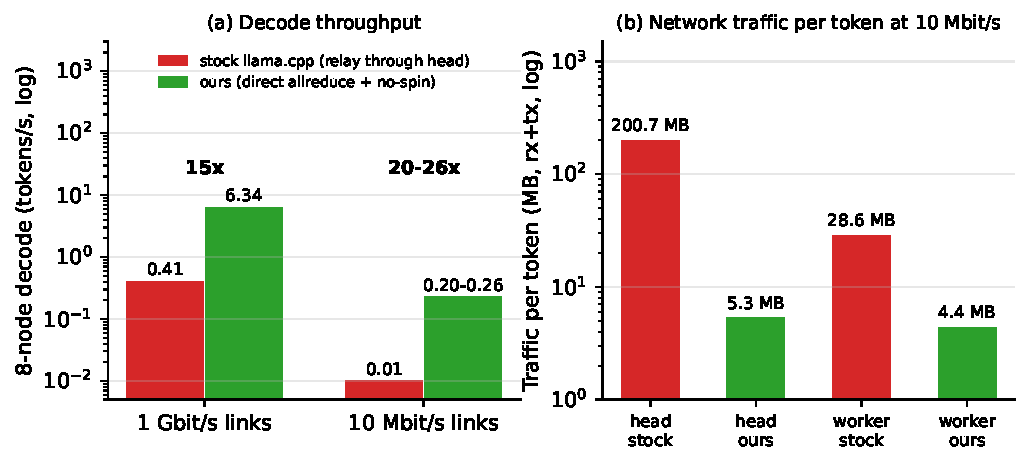
\includegraphics[width=0.95\textwidth]{figures/bandwidth_10mbps.pdf}
\caption{(a) 8-node decode throughput of stock \texttt{llama.cpp} and our version at 1~Gbit/s and 10~Mbit/s links (log scale). (b) Traffic per generated token at 10~Mbit/s.}
\label{fig:10mbps}
\end{figure}

Table~\ref{tab:10mbps} and Figure~\ref{fig:10mbps} show the result. The stock implementation relays every partial sum through the head, which then has to send and receive about 200~MB per token; its uplink runs at 8.9~Mbit/s, i.e.\ saturated, and a token takes about 100~s (0.01 tokens/s). With the direct allreduce the head moves only 5.3~MB per token, almost 40$\times$ less, and every worker exchanges 4.4~MB, matching Eq.~\ref{eq:rd}. Our version reaches 0.20--0.26 tokens/s in two runs, 20--26$\times$ faster than stock, a larger factor than at 1~Gbit/s (15$\times$). At 10~Mbit/s our version is bandwidth- and latency-bound as well: the workers' links carry about 5~Mbit/s per direction, and each of the $56 \times 3 = 168$ sequential exchange rounds per token needs about 10~ms just to serialize 12~KB at 10~Mbit/s. The experiment therefore confirms that the traffic reduction of the direct allreduce matters most when the network is slow, while on our Gigabit switch it is the removal of the head as a serial relay that counts.

\subsection{Optimizing Pipeline Parallelism}\label{sec:n8_9}

Since PP cannot speed up a single request, we tested the two mechanisms that let several stages work at the same time.

\paragraph{Chunked (pipelined) prefill.} If a prompt is split into $m$ micro-batches (\texttt{-ub}, the maximum number of tokens per chunk), stage $i$ can process chunk $j+1$ while stage $i+1$ processes chunk $j$. With $N$ equally fast stages and stage time $t$ per chunk, the prefill time drops from $mNt$ to $(m+N-1)t$, i.e.
\begin{equation}
S_{\text{pipe}} = \frac{mN}{m+N-1},
\label{eq:pipe}
\end{equation}
which is $16/7 \approx 2.3$ for $m=N=4$. \texttt{llama.cpp} enables this automatically when all devices support asynchronous computation and events, which the RPC backend does (the log shows ``pipeline parallelism enabled''). Table~\ref{tab:pp} shows that it works but yields far less than Eq.~\ref{eq:pipe}: a 128-token prompt split into four chunks of 32 tokens is processed 12\% faster on 4 PP nodes (4.68 vs.\ 4.16 tokens/s), while chunking alone has no effect on a single node (4.13 tokens/s). We believe, without having verified it with the timing log yet, that the activations between consecutive stages are still relayed through the head (\texttt{get\_tensor} followed by \texttt{set\_tensor}), which serializes most of the pipeline; letting the servers send activations to each other directly, as we did for the allreduce, is the natural next step.

\paragraph{Serving several requests.} During decoding the weights must be streamed from memory once per step regardless of how many sequences are processed, so for a memory-bound device the aggregate throughput with $B$ concurrent requests behaves like
\begin{equation}
X(B) \approx \frac{B}{T_{w} + B\, t_{c}},
\label{eq:batch}
\end{equation}
where $T_w$ is the time to stream the weights and $t_c$ the per-sequence compute time. It grows almost linearly while $B\,t_c \ll T_w$ and saturates at $1/t_c$. We measured it with \texttt{llama-batched-bench} (32-token prompt and 16 generated tokens per request, $B \in \{1,4,8\}$). As Figure~\ref{fig:pp} and Table~\ref{tab:pp} show, batching raises the aggregate decode throughput of a single node from 1.85 to 3.46 tokens/s and of 4-node PP from 1.83 to 3.24 tokens/s, i.e.\ PP benefits from batching exactly like a single node but is not better at it. Splitting the batch of 8 requests into four micro-batches of 2 (\texttt{-ub 2}) pipelines the decode steps across the stages and raises 4-node PP to 4.18 tokens/s (+29\%), the only PP configuration that beats a single node. 4-node TP, however, reaches 7.83 tokens/s with 8 requests.

\begin{table}[H]
\centering
\caption{Pipeline-parallel optimizations on 4 Raspberry Pi nodes.}
\label{tab:pp}
\begin{tabular}{@{}llc@{}}
\toprule
Experiment & Configuration & Throughput (tok/s) \\
\midrule
Prefill, 128-token prompt & Single node, \texttt{-ub 32} & 4.13 \\
 & PP, \texttt{-ub 128} (1 chunk) & 4.16 \\
 & PP, \texttt{-ub 32} (4 chunks) & \textbf{4.68} (+12\%) \\
\midrule
Aggregate decode, $B = 1 / 4 / 8$ & Single node & 1.85 / 3.40 / 3.46 \\
 & PP & 1.83 / 3.17 / 3.24 \\
 & PP, $B=8$, \texttt{-ub 2} (pipelined decode) & \textbf{4.18} (+29\%) \\
 & TP, untied, 4 threads & 4.26 / 6.46 / \textbf{7.83} \\
\bottomrule
\end{tabular}
\end{table}

\begin{figure}[H]
\centering
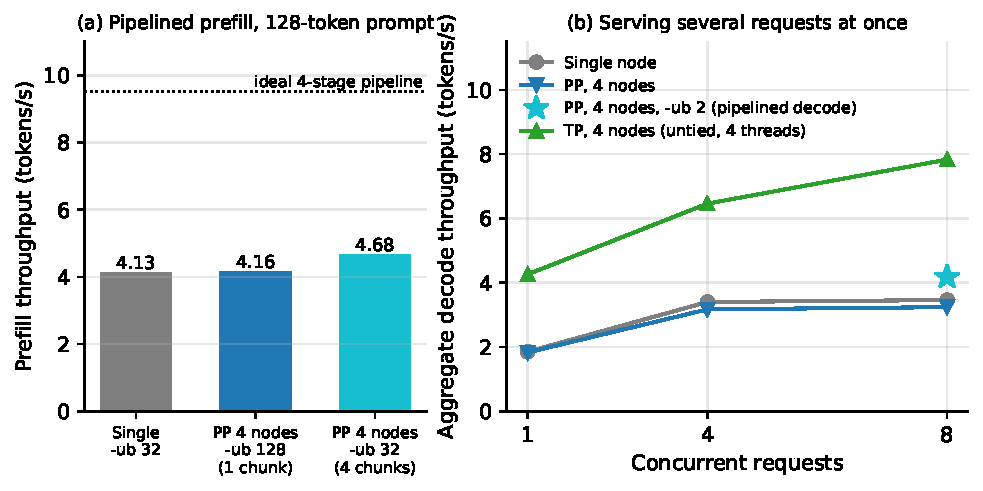
\includegraphics[width=0.95\textwidth]{figures/pp_pipeline_batching.pdf}
\caption{(a) Pipelined prefill on 4 PP nodes; the dotted line is the ideal speedup of Eq.~\ref{eq:pipe}. (b) Aggregate decode throughput when serving several requests at once.}
\label{fig:pp}
\end{figure}

\paragraph{Eight nodes.} With eight devices PP reaches 2.00 tokens/s decode and 4.06 tokens/s prefill with an even split, and 2.29 and 4.98 tokens/s when the RK3588 board receives four times as many layers as each Raspberry Pi (\texttt{-ts 1/1/1/1/1/1/1/4}). Since only one stage works at a time, the per-token time is the sum of the stage times, and moving layers to the fastest device is the only lever; the resource monitor confirms that every device is busy only 5--14\% of the time and that the network carries only the activations between stages (30~kB per token) and the logits to the head (513~kB per token).

On a cluster of small boards with a fast local network, TP is therefore better than PP for single requests, for prefill and for serving several requests. The real use of PP is capacity: it lets a model that does not fit into one board run at roughly single-board speed. Since TP also stores only $1/N$ of the layer weights per node, this advantage matters only for models where TP is not applicable (e.g.\ when the number of KV heads is not divisible by $N$).

\subsection{Heterogeneous Cluster}\label{sec:n8_10}

Real edge deployments mix devices of different speed. Table~\ref{tab:hetero} and Figure~\ref{fig:hetero} report experiments with one LubanCat-5 (RK3588) board.

\paragraph{The build matters more than the board.} With the generic Cortex-A72 build, the RK3588 board decodes at 5.84 tokens/s using its four big cores. Compiled for the Cortex-A76 (with dot-product instructions), it reaches 12.28 tokens/s decode and 48.75 tokens/s prefill, 2.1$\times$ and 6.5$\times$ more, and 6.7$\times$ the decode speed of a Raspberry Pi. Using all eight cores is slower (10.12 tokens/s) than using only the four big cores, because the parallel kernels wait for the slow Cortex-A55 cores.

\paragraph{Weighted splits.} With an even split, every node of a TP or PP group receives the same amount of work and the fast board waits for the slow ones: in a 2-node TP group of one Pi and the RK3588 board, the timing log shows the RK3588 board computing for 65~ms and then waiting 200~ms per token for the Pi. Both split modes accept a per-device proportion (\texttt{-ts}). For TP, the per-token time is determined by the slowest node,
\begin{equation}
T = \max_i \frac{w_i}{v_i}, \qquad \text{minimized by} \quad w_i = \frac{v_i}{\sum_j v_j},
\label{eq:weighted}
\end{equation}
where $w_i$ is the share of the work and $v_i$ the speed of node $i$. A split of 1:4 between the Pi and the RK3588 board raises TP decode from 3.24 to 7.00 tokens/s and prefill from 7.71 to 17.17 tokens/s; for PP, a 1:6 split raises decode from 3.07 to 5.52 tokens/s. At 8 nodes, however, an uneven tensor split collides with our direct allreduce: with \texttt{-ts 1/1/1/1/1/1/1/2} the partial tensors of the devices have different sizes, the direct path (which assumes equal sizes) is skipped, and the allreduce falls back to the relay through the head (92~MB sent by the head per token, 0.11 tokens/s; measured with busy-spinning dispatchers). Supporting uneven shards in the direct allreduce is therefore a prerequisite for weighted tensor-parallel splits beyond two nodes. Nevertheless, for this model every mixed configuration is slower than the RK3588 board alone (12.28 tokens/s), because the Pi adds more time than it saves: heterogeneous clusters are useful only when the model does not fit on the fastest device, and then the split must follow the device speeds.

\begin{table}[H]
\centering
\caption{Heterogeneous experiments with one LubanCat-5 (RK3588) board (``cat''); the head is a Raspberry Pi 400 in all cluster runs.}
\label{tab:hetero}
\begin{tabular}{@{}lcc@{}}
\toprule
Configuration & Prefill (tok/s) & Decode (tok/s) \\
\midrule
cat alone, generic A72 build, 4 big cores & 7.48 & 5.84 \\
cat alone, A76 build, 8 cores & 47.44 & 10.12 \\
cat alone, A76 build, 4 big cores & \textbf{48.75} & \textbf{12.28} \\
\midrule
TP, Pi + cat, even split & 7.71 & 3.24 \\
TP, Pi + cat, \texttt{-ts 1/4} & 17.17 & 7.00 \\
PP, Pi + cat, even split & 6.25 & 3.07 \\
PP, Pi + cat, \texttt{-ts 1/6} & 10.57 & 5.52 \\
TP, cat + 3 Pis, even split & 12.28 & 4.57 \\
PP, cat + 3 Pis, 128-token prompt, \texttt{-ub 32}, even split & 6.07 & 2.12 \\
PP, cat + 3 Pis, 128-token prompt, \texttt{-ub 32}, \texttt{-ts 1/12/1/1} & 13.12 & 3.47 \\
\bottomrule
\end{tabular}
\end{table}

\begin{figure}[H]
\centering
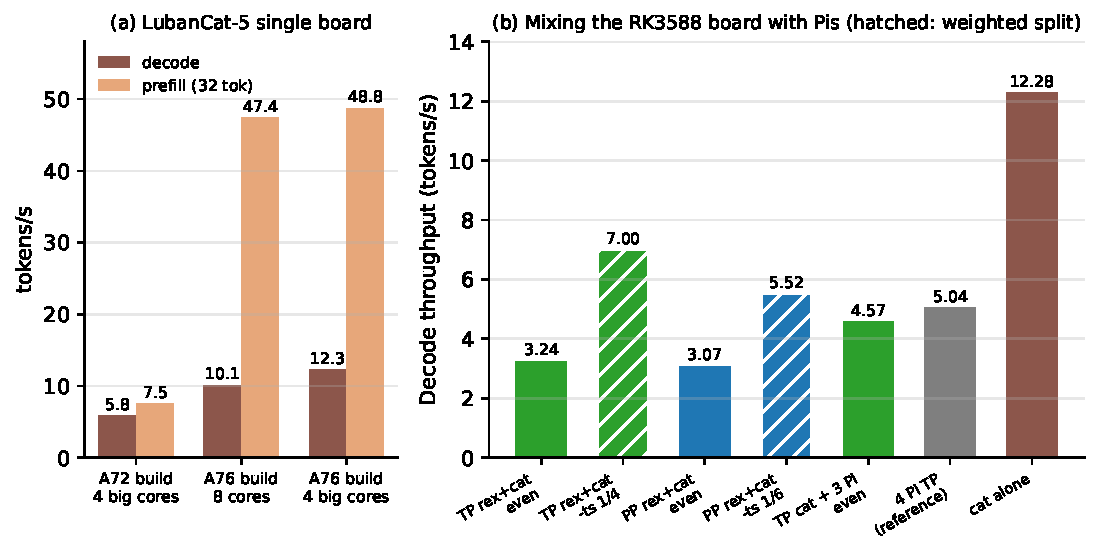
\includegraphics[width=0.98\textwidth]{figures/heterogeneous.pdf}
\caption{(a) The RK3588 board with different builds and core sets. (b) Mixing it with Raspberry Pis; hatched bars use a speed-proportional split.}
\label{fig:hetero}
\end{figure}

\subsection{Discussion: Connecting the Results Back to the Requirements}\label{sec:n8_11}

Table~\ref{tab:summary} summarizes the bottlenecks we found, the optimizations we applied and their measured effects. Regarding the requirements of Section~\ref{sec:n4_2}: the cluster runs a model by splitting both memory and compute across the boards (R1) on commodity hardware without accelerators (R2); our direct allreduce supports any power-of-two number of nodes up to 16 without re-slicing the model by hand and was verified on 2, 4 and 8 devices (R3); the timing log records computation, synchronization, transfer and idle time per token and per node, and the resource monitor records CPU, memory, network bytes and packets on every device in every run (R4); and every result is produced by a script in the public repository, with raw logs and timing logs checked in, and repeated runs agreeing within a few percent (R5).

\begin{table}[H]
\centering
\caption{Summary of bottlenecks, optimizations and measured effects (decode throughput in tokens/s unless noted).}
\label{tab:summary}
\small
\begin{tabular}{@{}p{2.2cm}p{4.7cm}p{4.6cm}p{3.0cm}@{}}
\toprule
Area & Bottleneck & Optimization & Effect \\
\midrule
Single device & Memory bandwidth (weights read at 70--85\% of measured bandwidth) & -- (motivates distribution) & 1.84 (Pi), 12.28 (RK3588) \\
TP & Allreduce relayed through the head (49.9 MB/token) & Direct peer-to-peer recursive-doubling allreduce & 4 nodes: 1.03 $\rightarrow$ 2.99 \\
TP & Tied output layer replicated on every node (80 ms/token/node) & Untied output layer (identical results) & 4 nodes: 2.99 $\rightarrow$ 4.85 \\
TP & Compute share per node becomes small & 4 threads per RPC server & 4 nodes: 4.85 $\rightarrow$ 5.04 \\
TP, slow network & Head relay saturates the head's 10 Mbit/s link (200 MB/token) & Direct allreduce (5.3 MB/token at the head) & 8 nodes at 10 Mbit/s: 0.01 $\rightarrow$ 0.20--0.26 \\
TP & Head CPU saturated by busy-spinning dispatchers (8 nodes: 94\% CPU, 470 ms idle per token on every node) & \texttt{GGML\_RPC\_NO\_SPIN} & 8 nodes: 1.62 $\rightarrow$ 6.34; prefill 13.4 $\rightarrow$ 16.2 \\
PP & Only one stage active per request & Chunked prefill (\texttt{-ub 32}) & prefill +12\% \\
PP & Same, with several requests & Batching + pipelined decode (\texttt{-ub 2}) & 3.24 $\rightarrow$ 4.18 \\
Network & DHCP timeouts reset the interfaces & Switch DHCP with MAC bindings + static addresses & no interruptions \\
Heterogeneity & Generic build lacks dot-product kernels & Build for Cortex-A76, pin to big cores & RK3588: 5.84 $\rightarrow$ 12.28 \\
Heterogeneity & Even split waits for the slowest node & Speed-proportional split (\texttt{-ts}) & Pi + RK3588 TP: 3.24 $\rightarrow$ 7.00; PP 8: 2.00 $\rightarrow$ 2.29 \\
\bottomrule
\end{tabular}
\end{table}

Two of our mid-term expectations turned out to be wrong, which is itself a useful result. We expected communication volume to be the main scaling bottleneck and planned to reduce it; on a switched Gigabit network the volume is small and the latency is low, and the dominant problems were implementation choices: who relays the synchronization, and which tensors are split. We also expected pipeline parallelism to be competitive for edge clusters because of its low communication volume; it is cheap, but without parallel work across stages it cannot be faster than one board.

% =====================================================
\section{Conclusions}\label{sec:n9}

\subsection{Summary}\label{sec:n9_1}
We deployed distributed LLM inference on a physical cluster of up to eight devices (seven Raspberry Pis and one RK3588 board) connected by a Gigabit switch, and studied it with two frameworks. Distributed Llama gives a tensor-parallel baseline of 1.97, 3.55 and 5.81 tokens/s on 1, 2 and 4 nodes. With \texttt{llama.cpp}, which supports both strategies, pipeline parallelism stays at single-node speed (1.84--2.00 tokens/s) for one request, while stock tensor parallelism falls to 1.03 tokens/s on 4 nodes and 0.41 tokens/s on 8 nodes because all synchronization is relayed through the head. Two independent instruments, a resource monitor on every device and a timing log inside every RPC server, let us find and remove three bottlenecks: the head relay (replaced by a direct recursive-doubling allreduce), the replicated tied output layer (removed by storing an identical untied copy), and the head's CPU being exhausted by busy-spinning RPC dispatcher threads at 8 nodes (fixed by a switch that makes them block). Tensor-parallel decode then scales to 3.46, 5.02 and 6.34 tokens/s on 2, 4 and 8 nodes (3.4$\times$ a single Raspberry Pi, 15.5$\times$ stock \texttt{llama.cpp} at 8 nodes) and prefill to 16.24 tokens/s, without any change in the model's output. With every link limited to 10~Mbit/s, the stock relay needs 200~MB per token at the head and reaches 0.01 tokens/s, while the direct allreduce needs 5.3~MB and reaches 0.20--0.26 tokens/s (20--26$\times$). For pipeline parallelism, chunked prefill and pipelined multi-request decoding give +12\% and +29\%, but tensor parallelism is better on every metric we measured. A heterogeneous RK3588 board is 6.7$\times$ faster than a Pi when compiled for its cores, and mixing devices requires speed-proportional splits.

Our answers to the research questions are: (RQ1) with a good implementation, decode throughput scales sub-linearly (3.4$\times$ on 8 nodes) and prefill better (3.9$\times$); (RQ2) TP is clearly better than PP on these devices, while PP is only useful for capacity; (RQ3) the bottleneck is memory bandwidth on one board and, on the cluster, the parts of the system that do not shrink with $N$ (the head relay, the unsplit output layer and the head's CPU), not network bandwidth, which is at most 25\% utilized; (RQ4) simple changes (a different allreduce, an untied model file, no busy-spinning, the thread count and a weighted split) improve throughput substantially without any loss of accuracy.

\subsection{Limitations}\label{sec:n9_2}
The 8-node configuration necessarily includes the RK3588 board, so we have no 8-node measurement with identical devices; the even split makes the RK3588 board wait for the Raspberry Pis, so an all-Pi cluster would behave similarly. We studied one model (Llama-3.2-3B-Instruct, Q4\_0); larger models that do not fit on one board, where pipeline parallelism and heterogeneous splits become essential, were not measured. Weighted tensor-parallel splits beyond two nodes currently fall back to the head relay, because our direct allreduce assumes equal shard sizes. The explanation for the limited gain of pipelined prefill is a hypothesis that we have not confirmed with the timing log. The resource monitor costs up to 2--3\% of throughput when all cores are busy. Each configuration was measured with one to two repetitions of \texttt{llama-bench}; repeated configurations agreed within a few percent, but we did not compute confidence intervals.

\subsection{Further Study Directions}\label{sec:n9_3}
The most promising next steps follow directly from our bottleneck analysis: supporting uneven shards in the direct allreduce, so that heterogeneous devices can be weighted in tensor parallelism at any cluster size; reducing the per-token head overhead $T_h$ in Eq.~\ref{eq:model} and the number of synchronization rounds, which together already take about half of each token at 8 nodes; sending pipeline activations directly between RPC servers instead of through the head, which Eq.~\ref{eq:pipe} suggests could more than double the pipelined prefill throughput; running models larger than one board's memory; and combining our communication optimizations with speculative decoding~\cite{leviathan2023fast} or KV cache compression~\cite{li2024surveykv}.

% =====================================================
\begin{thebibliography}{99}

% --- Core Architecture & Foundational Models ---
\bibitem{vaswani2017attention}
A.~Vaswani, N.~Shazeer, N.~Parmar, J.~Uszkoreit, L.~Jones, A.~N.~Gomez, L.~Kaiser, and I.~Polosukhin,
``Attention is All You Need,''
in \emph{Advances in Neural Information Processing Systems (NeurIPS)}, vol.~30, 2017.

\bibitem{huggingface}
Hugging Face,
``Hugging Face Model Hub,''
2024. [Online]. Available: \url{https://huggingface.co/models}

% --- Distributed & Edge Inference Systems ---
\bibitem{llamacpp}
G.~Gerganov \emph{et al.},
``llama.cpp: Port of Facebook's LLaMA model in C/C++ (with RPC support),''
GitHub repository, 2023. [Online]. Available: \url{https://github.com/ggml-org/llama.cpp}

\bibitem{distributedllama}
B.~Tadych,
``Distributed Llama,''
GitHub repository, 2024. [Online]. Available: \url{https://github.com/b4rtaz/distributed-llama}

\bibitem{buschmann2025}
P.~Buschmann \emph{et al.},
``LLMs on Edge: Network Traffic Characteristics of Distributed Inference under the Loupe,''
in \emph{Proceedings of the 2nd Workshop on Networks for AI Computing (NAIC)}, 2025.

\bibitem{zhao2024}
J.~Zhao \emph{et al.},
``POSTER: LLM-PQ: Serving LLM on Heterogeneous Clusters with Phase-Aware Partition and Adaptive Quantization,''
in \emph{Proceedings of the 29th ACM SIGPLAN Annual Symposium on Principles and Practice of Parallel Programming (PPoPP)}, 2024.

\bibitem{zhang2024edgeshard}
M.~Zhang, X.~Shen, J.~Cao, Z.~Cui, and S.~Jiang,
``EdgeShard: Efficient LLM Inference via Collaborative Edge Computing,''
\emph{IEEE Internet of Things Journal}, vol.~12, no.~10, pp.~13119--13131, 2025.

% --- Optimization Techniques: Speculative Decoding & KV Cache ---
\bibitem{leviathan2023fast}
Y.~Leviathan, M.~Kalman, and Y.~Matias,
``Fast Inference from Transformers via Speculative Decoding,''
in \emph{Proceedings of the 40th International Conference on Machine Learning (ICML)}, PMLR 202, pp.~19274--19286, 2023.

\bibitem{li2024surveykv}
H.~Li, Y.~Li, A.~Tian, T.~Tang, Z.~Xu, X.~Chen, N.~Hu, W.~Dong, Q.~Li, and L.~Chen,
``A Survey on Large Language Model Acceleration based on KV Cache Management,''
\emph{arXiv preprint arXiv:2412.19442}, 2024.

% --- Baseline Parallelism Literature ---
\bibitem{shoeybi2019}
M.~Shoeybi \emph{et al.},
``Megatron-LM: Training Multi-Billion Parameter Language Models Using Model Parallelism,''
\emph{arXiv preprint arXiv:1909.08053}, 2019.

\end{thebibliography}
% =====================================================
\appendix
\section{Final Presentation Slides}\label{app:slides}
The slides of our final presentation follow on the next pages (two slides per page).
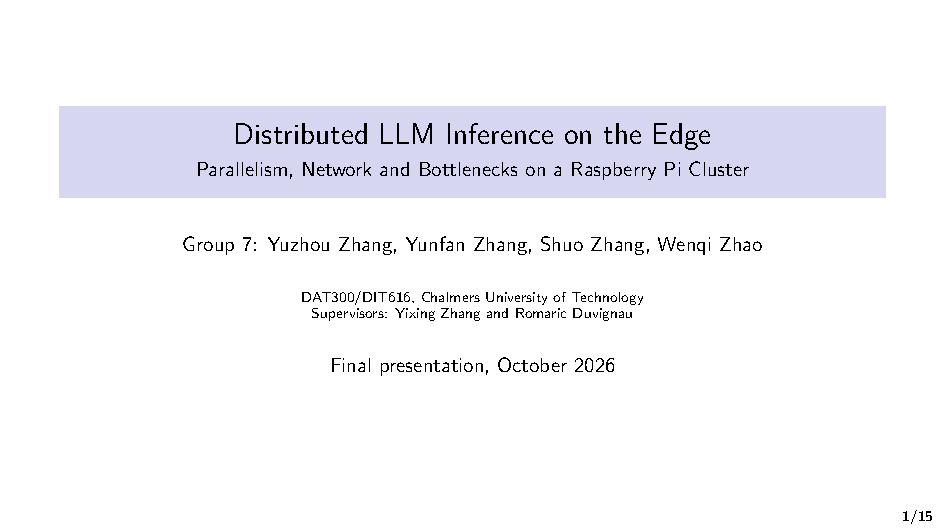
\includepdf[pages=-, nup=1x2, frame, delta=0 8mm, pagecommand={}]{slides.pdf}

\end{document}